\documentclass{beamer}

\usepackage{amsmath}
\usepackage{amssymb}
\usepackage{graphicx}
\usepackage{subcaption}
\usepackage{float}
\usepackage{multirow}
\usepackage{alphalph}
\usepackage{listings}

\usepackage{appendixnumberbeamer}
\usetheme{Frankfurt}
%\xdefinecolor{maroon}{cmyk}{0.15,1.00,0.39,0.69}
%\xdefinecolor{maroon}{cmyk}{0.27,0.86,0.60,0.30}
%\xdefinecolor{maroon}{cmyk}{0.000,1.00,1.00,0.498}
\usecolortheme[RGB={80,0,0}]{structure}

% Shortcut commands
% My Shortcut Commands
\newcommand{\fig}[1]{Fig.~\ref{#1}}                      % figure
\newcommand{\tbl}[1]{Table~\ref{#1}}                     % table

\newcommand{\be}{\begin{equation*}}   % numbered equation
\newcommand{\ee}{\end{equation*}}

\newcommand{\benum}{\begin{equation}}   % numbered equation
\newcommand{\eenum}{\end{equation}}

\newcommand{\bea}{\begin{eqnarray*}}  % numbered equation array
\newcommand{\eea}{\end{eqnarray*}}

\newcommand{\beanum}{\begin{eqnarray}}  % numbered equation array
\newcommand{\eeanum}{\end{eqnarray}}

\newcommand{\eqt}[1]{Eq. (\ref{#1})}  % Reference to one equation
\newcommand{\eqts}[1]{Eqs. (\ref{#1})}  % Reference to multiple equations 

\newcommand{\B}[1]{\ensuremath{b_{#1} }}			% B with a sub scripted argument

\newcommand{\R}[1]{\ensuremath{\mathbf{R}_{#1}}}
\newcommand{\D}{\ensuremath{ \mathbf{D}_* }}
\newcommand{\I}{\ensuremath{ \mathbf{I} }}
\newcommand{\M}{\ensuremath{ \mathbf M}}

\newcommand{\p}{\ensuremath{ \partial}}			% shortcut partial derivative symbol

\newcommand{\abs}[1]{\ensuremath{\left\lvert #1 \right\rvert}}  % absolute value of argument (variable bar size)
\newcommand{\norm}[1]{\ensuremath{\left\lVert #1 \right\rVert}}  % norm of argument, varaible size


% Equation Punctuation
\newcommand{\pec}{\, ,}
\newcommand{\pep}{\, .}
\setbeamertemplate{footline}{
\leavevmode%
\hbox{\hspace*{-0.06cm}
\begin{beamercolorbox}[wd=.45\paperwidth,ht=2.25ex,dp=1ex,center]{author in head/foot}%
	\usebeamerfont{author in head/foot}Maginot%~~(\insertshortinstitute)
\end{beamercolorbox}%
\begin{beamercolorbox}[wd=.3\paperwidth,ht=2.25ex,dp=1ex,center]{section in head/foot}%
PhD Defense %\usebeamerfont{section in head/foot}\insertshorttitle
\end{beamercolorbox}%
\begin{beamercolorbox}[wd=.25\paperwidth,ht=2.25ex,dp=1ex,right]{section in head/foot}%
	\usebeamerfont{section in head/foot}April 2015\hspace*{2em}
	\insertframenumber{} / \inserttotalframenumber\hspace*{2ex}
\end{beamercolorbox}}%
\vskip0pt%
}
\beamertemplatenavigationsymbolsempty
\beamertemplatetransparentcovered

\setbeamertemplate{bibliography item}[text]

\title{PhD Defense \\ Higher Order Grey Thermal Radiative Transfer}
\author{Peter Maginot}\institute{Texas A\&M University- Department of Nuclear Engineering}
\date{April 2015}


\newif\ifplacelogo % create a new conditional
\placelogotrue % set it to true
\logo{\ifplacelogo
\includegraphics[height=1cm]{CSGF_vert.pdf} \hspace{3.5in} 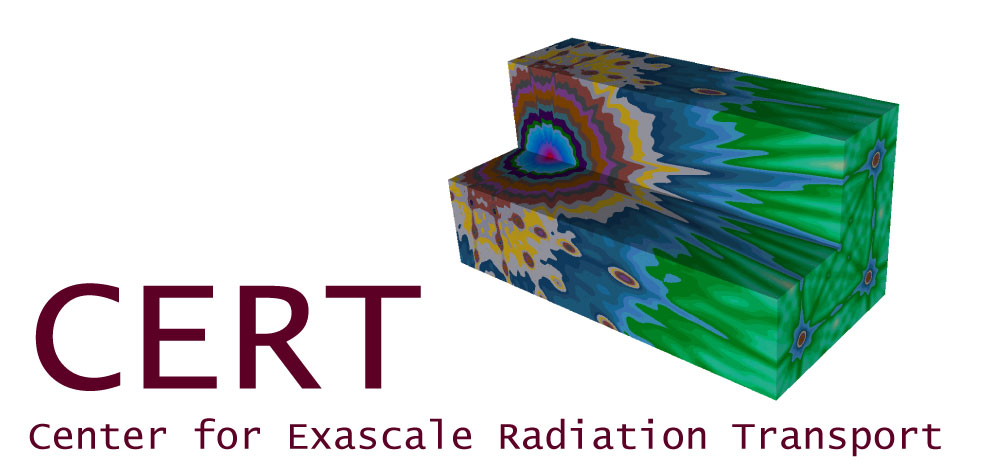
\includegraphics[height=1cm]{cert-logo}\fi}

\begin{document}
%---------------------------------------------------------------------------------------------
\placelogotrue
\begin{frame}
\titlepage


\end{frame}

%---------------------------------------------------------------------------------------------

\placelogofalse
%---------------------------------------------------------------------------------------------
\begin{frame}
\frametitle{Outline}
\tableofcontents[hideallsubsections]
%\begin{enumerate}
%\item Spatially Varying Cross Section Problems
%\item Low Order DSA for High Order DFEM Transport
%\item Strictly Non-Negative Bilinear Scheme for Unstrutured Quads
%\end{enumerate}
\end{frame}

\section{New Results}

\subsection{Grey thermal radiative transfer}
\begin{frame}
\frametitle{New for Today}
Results
\begin{itemize}
\item Su-Olson Problem
\item Manufactured Solutions
\item High Resolution Marshak Wave Simulations
\end{itemize}
Coding
\begin{itemize}
\item Arbitrary DFEM trial space degree
\item Arbitrary SDIRK schemes
\item MIP diffusion operator for grey radiative transfer
\item Done in C++ with lots of bells and whistles
\end{itemize}
\end{frame}

\begin{frame}
\frametitle{Didn't Have All That Capability at Prelim?}

\begin{itemize}
\item Was in MATLAB, now in C++
\begin{itemize}
\item About 19,000 lines of C++ (PDT+TAXI-STAPL is about 106k lines)
\item Code leverages outside packages: CMAKE, PETSc, Eigen, TinyXml
\item DARK\_ARTS can be read by / used by someone other than me
\item $>20 \times$ speed-up compared to MATLAB
\end{itemize}
\item Used S2SA, now use MIP
\item Incorporated extensive unit testing
\item Framework for multi-frequency in place
\end{itemize}

\end{frame}

\section{Contributions}
\subsection{Contributions}
\begin{frame}
\frametitle{Contributions to Discrete Ordinates Transport}
\begin{enumerate}
%
\item Lumping framework (prelim)
\item Spatially varying cross section treatment (prelim)
\item Application of higher order DFEM to grey TRT (new)
\end{enumerate}

\end{frame}
%
\subsection{Prelim Contributions}
\begin{frame}
\frametitle{Lumping Framework}
\begin{itemize}
\item Introduced quadrature based self-lumping (SL) schemes for discrete ordinates
\item Improved robustness versus traditional lumping (TL)
\item Considered non-equally spaced DFEM interpolation points
\item Demonstrated that SL schemes increased in accuracy with increased $P$
\item Demonstrated that $TL$ were at most third order convergent in space, for all $P$
\end{itemize}
\end{frame}
%
\begin{frame}
\frametitle{Spatially Varying Cross Section}
%
\begin{itemize}
\item Demonstrated poor accuracy of cell-wise constant approximation
\item Demonstrated non-physical interaction rate of cell-wise constant schemes
\item Modified SL schemes to account for within cell cross section variation (SLXS)
\item SLXS schemes retained $P+1$ $L^2$ convergence for pure absorber and fuel depletion problem
\end{itemize}

\end{frame}



\subsection{Grey TRT}
\begin{frame}
\frametitle{Grey TRT}
\begin{enumerate}
\item Adapting MIP diffusion operator to TRT linearization
\item Numerical Results
\begin{itemize}
\item Validation (Su-Olson problem)
\item Order of convergence (Method of Manufactured Solutions)
\item High resolution capability (Marshak wave problem)
\end{itemize}
\end{enumerate}
\end{frame}

\section{MIP for TRT}
\subsection{Analytic Equations}
\begin{frame}
\frametitle{Grey TRT Equations}
\bea
\frac{1}{c} \frac{\partial I}{\p t} + \mu_d \frac{\p I}{\p x}  + \sigma_t I &=&  2\pi \int_{-1}^{1}{ \sigma_s(\mu'\to\mu_d) I  d\mu }+ \sigma_a B + S_I\\
C_v \frac{\p T}{\p t} &=&   \sigma_a \left( \phi- 4\pi B   \right) + S_T
\eea
\centering
\begin{itemize}
\item $I(x,\mu_d,t)$ - intensity $\left[ \frac{energy}{area-time-ster} \right]$
\item $\phi(x,t)$ - angle integrated intensity $\left[ \frac{energy}{area-time} \right]$
\item $T(x,t)$ - temperature
\item $\sigma_{a}$ - absorption opacity  $\left[ {length}^{-1} \right]$
\item $\sigma_{s}$ - scattering opacity  $\left[ {length}^{-1} \right]$
\item $C_v$ - heat capacity $\left[ \frac{energy}{volume-temperature} \right]$
\item $B$ - Planck function $\left[ \frac{energy}{area-time-ster} \right]$
\end{itemize}
\end{frame}

\begin{frame}
\frametitle{Solution Methodology}
\begin{enumerate}
\item Linearize Planckian in temperature
\item Expand Planckian in $P$ degree trial space
\item Use temperature equation to make radiation equation linear (for a given temperature iterate)
\item Ignore non-linearity of material properties
\item Assume SDIRK time integration
\item Iterate for temperature using damped Newton iteration, with time step control
\end{enumerate}
\end{frame}

\subsection{Spatially Analytic}
\begin{frame}
\frametitle{Spatially Analytic Linearized TRT Radiation Equation}
\benum
\mu_d \frac{\partial I_i}{\partial x} + \sigma_{\tau,i} = \frac{1}{4\pi} \sigma_s \phi_i + \frac{1}{4\pi}\nu_i \sigma_a \phi_i + \xi_i 
\label{eq:analytic_pseudo_i}
\eenum
\begin{subequations}
\benum
\nu_i = \frac{ 4\pi a_{ii} \Delta t \sigma_a D_*}{C_v + 4\pi a_{ii} \Delta t  \sigma_a D_*} 
\label{eq:analytic_nu}
\eenum
\benum
\sigma_{\tau,i} = \frac{1}{a_{ii} \Delta t c} + \sigma_t 
\label{eq:tau_i_analytic}
\eenum
\begin{itemize}
\item $a_{ii}$ is an SDIRK constant
\item $D_*$ is Planck derivative:
\be 
D_* = \frac{\p B}{\p T}\bigg \lvert_{T=T_*} 
\ee
\end{itemize}
%\begin{multline}
%\xi_i = \sigma_a B_* + S_I +  \frac{1}{a_{ii} \Delta t c} I_n + \frac{1}{a_{ii} c} \sum_{j=1}^{i-1}{a_{ij} k_{I,j}}  + \dots  \\ 
%\sigma_a D_*\left(1 + \frac{4\pi a_{ii} \Delta t}{C_v} \sigma_a D_*  \right)^{-1} 
%\left( T_n - T_* + \Delta t \sum_{j=1}^{i-1}{a_{ij} k_{T,j}} +  \dots \right.\\
%\left.   \frac{a_{ii} \Delta t }{C_v}  \left( S_T -  4\pi  \sigma_a B_*   \right) \right) 
%\end{multline}
\end{subequations}
\end{frame}

\subsection{Spatially Discretized}
\begin{frame}
\frametitle{Spatially Discretized Equations}
\be
\mu_d\mathbf{G} \vec{I}_i + \overline{\overline{\mathbf R}}_{\sigma_{\tau},i}\vec{I}_i = \frac{1}{4\pi}\R{\sigma_s}\vec{\phi}_i + \frac{1}{4\pi}\overline{\overline{\mathbf \nu}}_i \R{\sigma_a}\vec{\phi}_i + \overline{\overline{\mathbf \xi}}_{d,i} + \mu_d\vec{f}I_{in,i}
\ee
\begin{itemize}
\item $\mathbf{G}$ - local gradient operator (for $\mu_d > 0$)
\be
\B{i}(1)\B{j}(1) - \int_{-1}^1{\frac{\p \B{i}}{\p s}\B{j}(s)~ds} \pep
\ee
\item $\vec{f}$ - upwinding term 
\be
\vec{f}_i = \left\{ 
\begin{array}{ll}
\B{i}(-1)  & \text{  for } \mu_d>0 \\
-\B{i}(1)  & \text{  for } \mu_d<0 
\end{array}\right.
\ee
\item $\mathbf{R}_{\sigma_t}$ - reaction matrix for material property $f$
\be
\frac{\Delta x}{2}\int_{-1}^1{\sigma_t(s)\B{i}(s)\B{j}(s)~ds} \pep
\ee
\end{itemize}
%with 
%\bea
%\Delta x &=&  x_{i+1/2} - x_{i-1/2} \\
%x &=& x_i + \frac{\Delta x}{2}s 
%\eea
\end{frame}

\begin{frame}
\frametitle{More Terms}
\bea
\overline{\overline{\mathbf \nu}}_i &=& 4\pi \Delta t a_{ii} \R{\sigma_a} \D \left[\mathbf{I} + 4\pi\Delta t a_{ii}\R{C_v}^{-1}\R{\sigma_a}\D  \right]^{-1}\R{C_v}^{-1}
\\
\overline{\overline{\mathbf R}}_{\sigma_{\tau},i} &=& \R{\sigma_t} + \frac{1}{c\Delta t a_{ii}}\M \pec
\eea
\begin{itemize}
\item $\mathbf{I}$ - $N_P \times N_P$ identity matrix, $N_P = P+1$ 
\item $\M$ - mass matrix
\item $\D$ - diagonal matrix of Planck derivatives
\be
\mathbf{D}_{*,ii} = \frac{d B}{d T} \bigg \lvert_{T = T_{i,*}} \pep
\ee 
\end{itemize}
\end{frame}

\subsection{What is D}
\begin{frame}
\frametitle{MIP Diffusion Coefficient}
MIP diffusion operator defined for a problem of the form:
\be
\nabla \widetilde{D} \nabla \phi + \widetilde{\Sigma_a} \phi = S
\ee
\vspace{-0.2in}
\begin{itemize}
\item Need $\widetilde{D}$ point evaluations (cell edges)
\item Need $\R{\widetilde{\Sigma}_a}$
\item Spatially discretized TRT equations only give
\bea
\R{\widetilde{\Sigma}_t} &=& \overline{\overline{\mathbf R}}_{\sigma_{\tau},i} = \R{\sigma_t} + \frac{1}{c\Delta t a_{ii}}\M \\
\R{\widetilde{\Sigma}_s} &=& \overline{\overline{\mathbf \nu}}_i \R{\sigma_a} + \R{\sigma_s}
\eea
\end{itemize}
If  the spatially analytic linearization and spatially discretized linearization yield the same $\R{\widetilde{\Sigma}_t}$ in theory we can use MIP accelerator

\end{frame}

\begin{frame}
\frametitle{Equivalence for $\widetilde{\Sigma}_t$}
If we establish 
\be
\overline{\overline{\mathbf R}}_{\sigma_{\tau,i}} = \R{\sigma_{\tau,i}} \pec
\ee
we may then evaluate
\be
\widetilde{D} = \frac{1}{3\widetilde{\Sigma}_t} \pep
\ee
at all necessary points.
\\
\vspace{0.2in}
By definition:
\be
\R{\sigma_{\tau,i},jk} = \frac{\Delta x}{2} \int_{-1}^{1}{\B{j}(s) \B{k}(s) \left( \sigma_t(s) + \frac{1}{c a_{ii} \Delta t}  \right)~ds}
\ee
\end{frame}

\begin{frame}
\frametitle{Equivalence for $\widetilde{\Sigma}_t$}
Likewise
\bea
\overline{\overline{\mathbf R}}_{\sigma_{\tau,i}} &=& \frac{1}{a_{ii} c \Delta t} \M + \R{\sigma_t} \\
\overline{\overline{\mathbf R}}_{\sigma_{\tau,i}} &=& \frac{1}{a_{ii} c \Delta t} \frac{\Delta x}{2} \int_{-1}^1{\B{j}(s) \B{k}(s) ~ds} + \frac{\Delta x}{2} \int_{-1}^1{ \sigma_t(s) \B{j}(s) \B{k}(s)~ds} \\
\overline{\overline{\mathbf R}}_{\sigma_{\tau,i},jk} &=& \frac{\Delta x}{2} \int_{-1}^1{ \left(\frac{1}{a_{ii} c \Delta t} + \sigma_t(s)  \right) \B{j}(s) \B{k}(s)~ds} \\
& & ~~~~ \therefore  \overline{\overline{\mathbf R}}_{\sigma_{\tau,i},jk} = \R{\sigma_{\tau,i},jk}
\eea
This does not hold for $\widetilde{\Sigma}_a$, unless using SLXS or cell-wise constant schemes.  For generality, we define:
\be
\R{\widetilde{\Sigma}_a} = \overline{\overline{\mathbf R}}_{\sigma_{\tau,i}}  - \left( \R{\sigma_s} + \overline{\overline{\nu}}_i \R{\sigma_a} \right) 
\ee
\end{frame}

\begin{frame}
\frametitle{MIP Iterative Effectiveness}
\centering
Iteration Count for Upcoming Results
\footnotesize
\begin{tabular}{|c|c|c|c|}
\hline
Problem Description & Scheme & Average DSA+SI & Average SI \\
{}									&				 &  Iterations & Iterations  \\
\hline
MMS Constant Time	 & Cubic 			 & 1.6 & 2.3 \\
8 cells 						& SLXS Lobatto & {} & {} \\
\hline
MMS1 						& Quadratic 		& 2.0 & 13.5 \\
2 cells 				& SLXS Gauss 		& {}  & {} \\
\hline
MMS2 						& Linear	 & 1.0 & 2.7 \\
2 cells 					& SLXS Gauss & {} & {} \\
\hline
MMS Constant Space 									& Quartic 				 & 17.0 & 39.0 \\
Alexander 3-3, $\Delta t=1$					& SLXS Lobatto 			& {}  & {} \\
\hline
MMS Constant Space 										& Quartic 				 & 2.3 & 4.9 \\
Alexander 3-3, $\Delta t=\frac{1}{128}$	& SLXS Lobatto 			& {}  & {} \\
\hline
Marshak Wave 									&  Linear			 & 2.1 & 2.9 \\
20 cells, largest $\Delta t$	& SLXS Lobatto & {} 		 & {} \\
\hline
\end{tabular}
\end{frame}

\begin{frame}
\frametitle{Designed Optically Thick Problem}
$S_8$, 50 cells, P1 SLXS Lobatto, IE SDIRK, initially cold slab with $T=0.5$.
Incident current of 100 on LHS, vacuum RHS.
\centering
\bea
a=&c&=1 \\
C_v &=& 0.05\\
\sigma_a& = &\frac{5000}{T^2} \\
\sigma_s &=& 0 \\
x&\in&[0,100]\\ 
t&\in&[0,5] \\ 
\Delta t_{max} &=& 0.1 \\
\eea
\footnotesize
\begin{tabular}{|c|c|}
\hline	
Iterative Strategy		& Average Iterations  \\
\hline
SI+MIP				&   2.5  \\ 
\hline
SI  &   4460.7 \\
\hline
\end{tabular}
%
\end{frame}

\section{Su-Olson Problem}
\subsection{Commonalities}

\begin{frame}
\frametitle{Solution Algorithm}
\lstinputlisting[	basicstyle = \scriptsize,
									frame = none,
									label = lst:pseudo_code]{presentation_iteration_pseudo_code.txt}
\end{frame}

\begin{frame}
\frametitle{Numerical Methods}
\begin{enumerate}
\item {\bf TL}- traditional lumping, equally spaced DFEM interpolation points, volume average $C_v$ and $\sigma$, for historical comparison 
\item {\bf SL Lobatto}- self-lumping, Lobatto DFEM interpolation points, volume average $C_v$ and $\sigma$ 
\item {\bf SL Gauss}- self-lumping, Gauss DFEM interpolation points, volume average $C_v$ and $\sigma$  
\item {\bf SLXS Lobatto}- self-lumping incorporating spatial variation of material properties, Lobatto DFEM interpolation points 
\item {\bf SLXS Gauss}- self-lumping incorporating spatial variation of material properties, Gauss DFEM interpolation points
\end{enumerate}
\end{frame}

\subsection{Su Olson}
\begin{frame}
\frametitle{Su-Olson Description}
\begin{itemize}
\item Initially cold (absolute zero) half space
\item Volumetric source near origin for a finite period of time
\item Constant opacity
\item $C_v = \alpha T^3$
\begin{itemize}
\item $C_v$ assumption causes TRT equations to be linear in $I$ and $T^4$/material energy density
\item Computationally challenging if not tracking material energy density(IMC)
\item We impose
\end{itemize}
\be
C_v = \epsilon + \alpha T^3
\ee
\end{itemize}
We choose $\sigma_a = 1,~\sigma_s = 0,~a=c=1,~\& \alpha = 4$. 
We truncate the half-space to be $x\in[0,10]$ and the source is located in $x\in[0,0.5]$.
\end{frame}


\begin{frame}
\frametitle{Su-Olson Results with $S_2$}

\begin{columns}[t]
\column{0.48\textwidth}
\centering
%\begin{figure}[!htp]
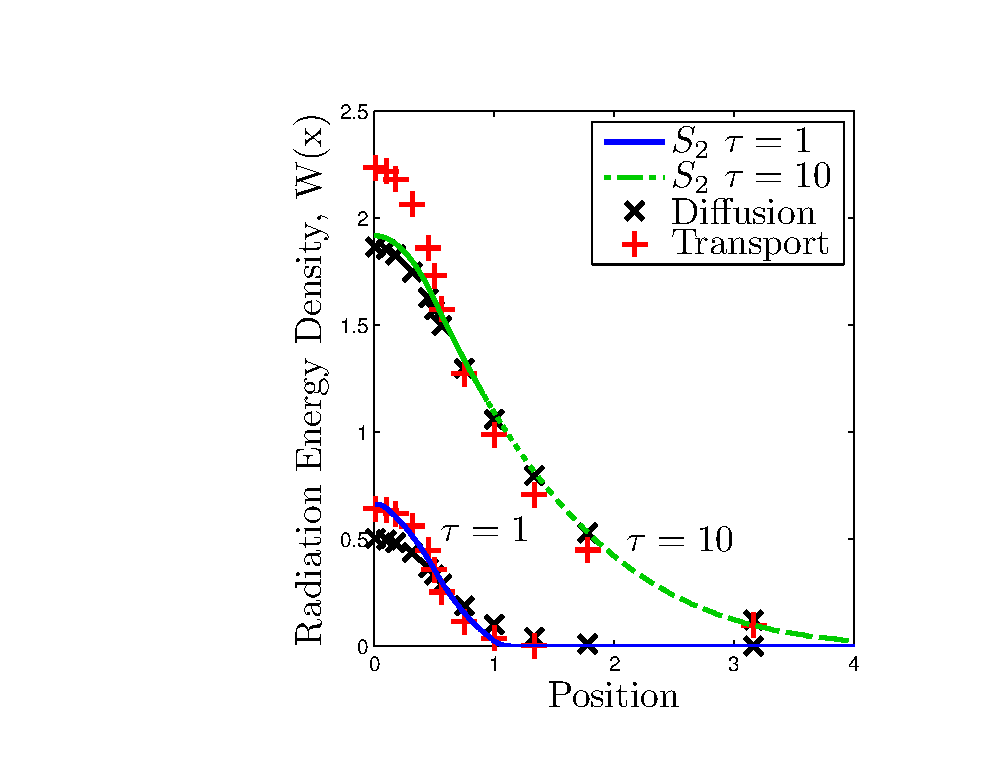
\includegraphics[width=5cm,trim=1.75in  0.5in 0.75in 0.5in,clip=true]{../chapter6_grey_radtran/Dissertation_Data/Su_Olson_S2_Radiation_Energy.pdf}
%\caption{$S_2$ radiation energy density profile for Su-Olson problem.}
%\label{fig:su_olson_s2_rad}
%\end{figure}
%\begin{figure}[!hbp]
%\centering
\column{0.48\textwidth}
\centering
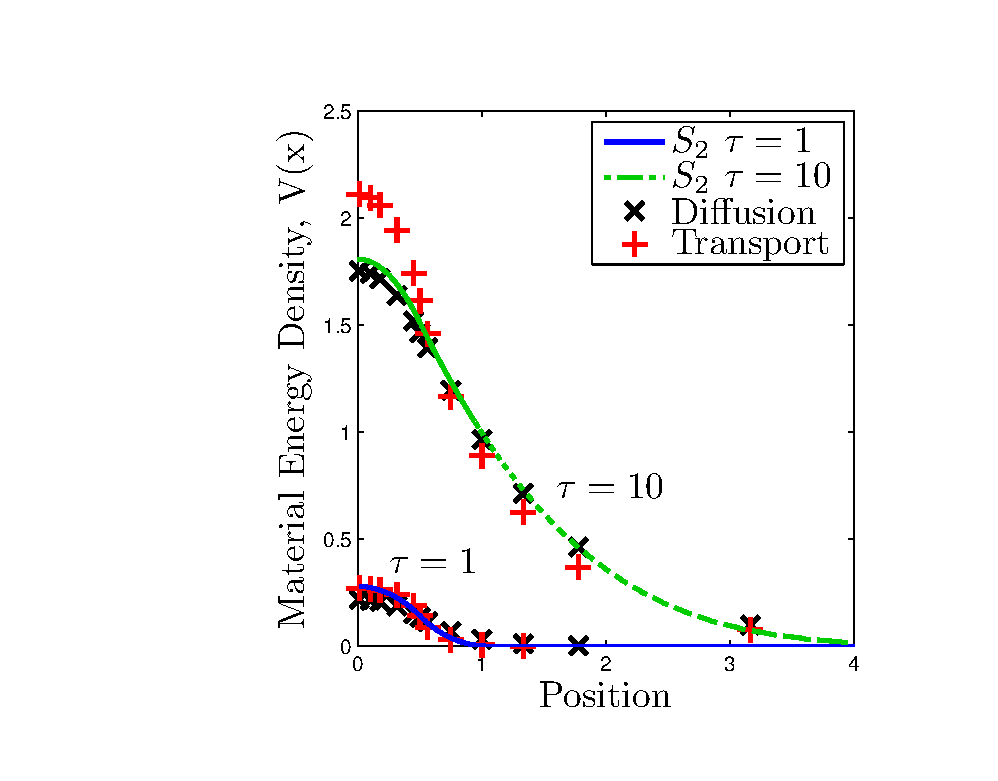
\includegraphics[width=5cm,trim=1.75in  0.5in 0.75in 0.5in,clip=true]{../chapter6_grey_radtran/Dissertation_Data/Su_Olson_S2_Material_Energy.pdf}
%\caption{$S_2$ material energy density profile for Su-Olson problem.}
%\label{fig:su_olson_s2_mat}
%\end{figure}
\end{columns}
Calculated using 200 cells, linear SLXS Lobatto, $\Delta t = 10^{-3}$
\end{frame}

\begin{frame}
\frametitle{Su-Olson Results with $S_8$}
\begin{columns}[t]
\column{0.48\textwidth}
\centering
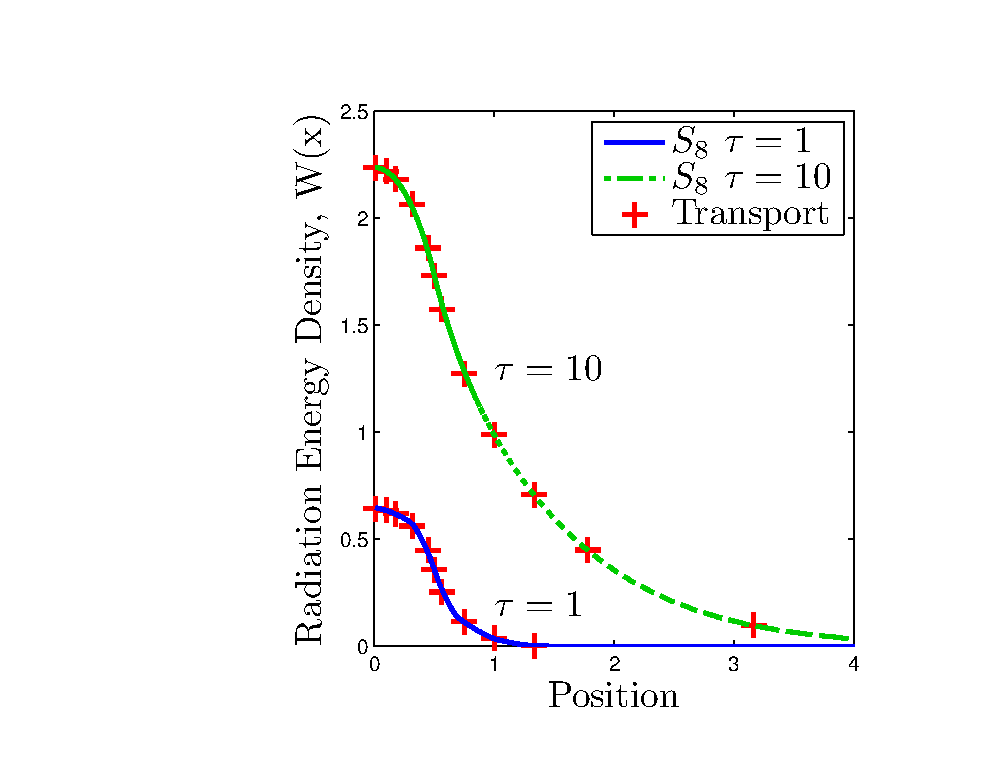
\includegraphics[width=5.5cm,trim=1.75in  0.5in 0.75in 0.5in,clip=true]{../chapter6_grey_radtran/Dissertation_Data/Su_Olson_S8_Radiation_Energy.pdf}
%\caption{$S_2$ radiation energy density profile for Su-Olson problem.}
%\label{fig:su_olson_s2_rad}
\column{0.48\textwidth}
\centering
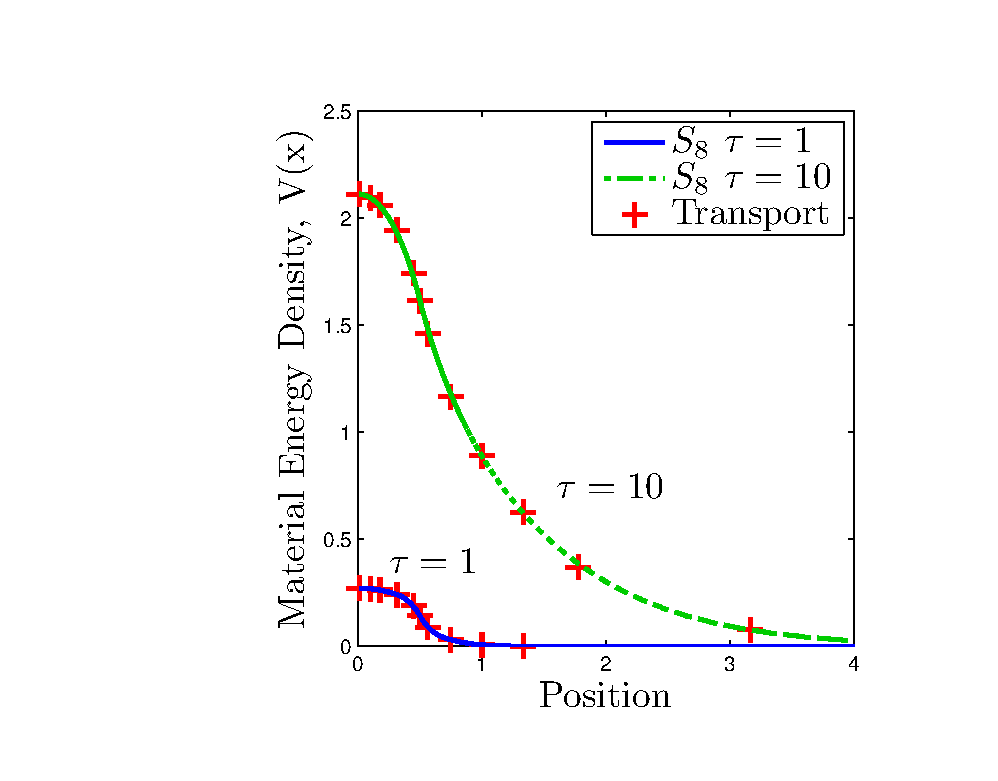
\includegraphics[width=5.5cm,trim=1.75in  0.5in 0.75in 0.5in,clip=true]{../chapter6_grey_radtran/Dissertation_Data/Su_Olson_S8_Material_Energy.pdf}
%\caption{$S_2$ material energy density profile for Su-Olson problem.}
\end{columns}
Calculated using 200 cells, linear SLXS Lobatto, $\Delta t = 10^{-3}$
\end{frame}

\section{MMS}
\subsection{MMS}

\begin{frame}
\frametitle{Error Measures}
\bea
E_{\phi} &=& \sqrt{\sum_{c=1}^{N_{cell}}{ \frac{\Delta x}{2} \sum_{q=1}^{N_{qf}}{ w_q \left(\widetilde{\phi}(s_q , t_{end}) - \phi(s_q,t_{end})  \right)^2 } } } \\
E_{\phi_A} &=& \sqrt{
\sum_{c=1}^{N_{cell}}{ 
\frac{\Delta x}{2} 
\left( 
\frac{1}{2}\sum_{q=1}^{N_{qf}}{ w_q \widetilde{\phi}(s_q , t_{end})}  - \frac{1}{2}\sum_{q=1}^{N_{qf}}{ w_q \phi(s_q , t_{end})} 
\right)^2 
} 
} 
\eea
\vspace{0.2in}
$E_T$ and $E_{T_A}$ are defined analogously.  $N_{qf} = 2P+ 7$, Gauss quadrature
\end{frame}

\begin{frame}
\frametitle{Choice of MMS}
Elect to use separable solution of the form
\beanum
I_d(x,\mu_d,t) &=& M(\mu_d) F(t) W_I(x) \\
T(x) &=& F(t) W_T(x) \\
\phi(x) &=& C_M F(t) W_I(x) \\
C_M &=& \sum_{d=1}^{N_{dir}} { w_d M(\mu_d) }
\eeanum
\end{frame}


\begin{frame}
\frametitle{SDIRK Order of Convergence}
\bea
M(\mu_d) &=& \frac{1}{4\pi} \\
W_I(x) &=& \frac{10}{4\pi} \\
W_T(x) &=&  10 \\
F(t) &=& 45 \cos\left( \pi t \right) + 46 \\
t &\in&[0,1] \\
\sigma_s &=& 0.1\\
\sigma_a &=& 2.5\\
C_v &=& 0.2 \\
x &\in & [0,10]
\eea
10 equally-spaced cells, quartic SLXS Gauss
\end{frame}

\begin{frame}
\frametitle{SDIRK Order of Convergence}
\begin{columns}[t]
\column{0.5\textwidth}
\centering
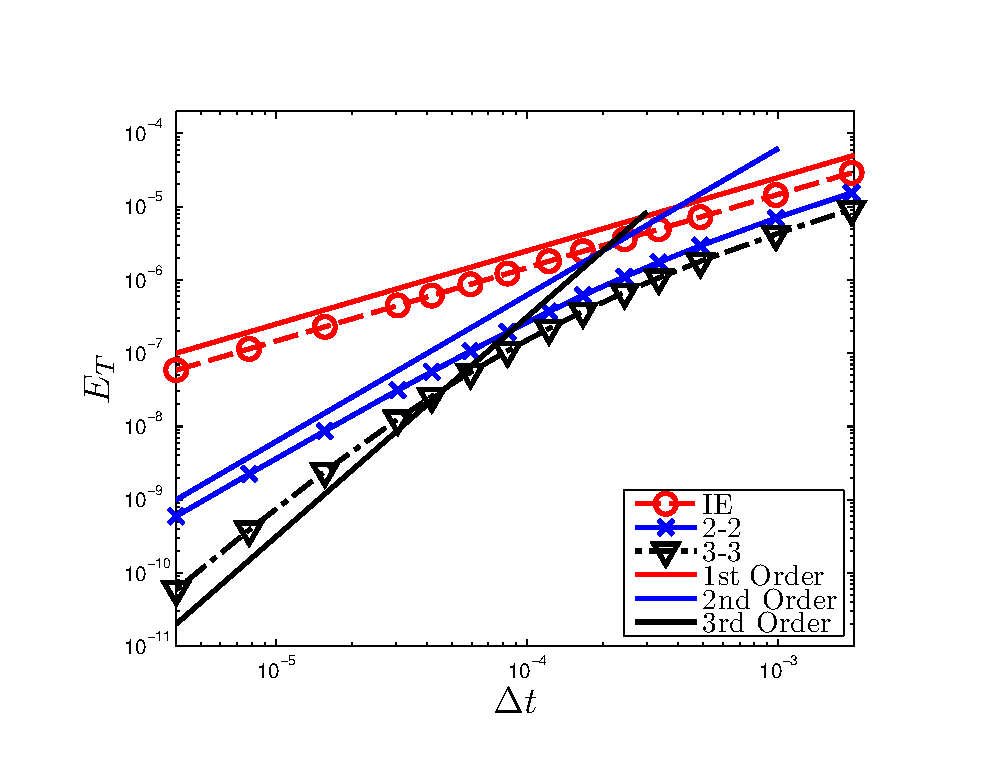
\includegraphics[width=\textwidth,trim=0.25in  0.2in 0.75in 0.5in,clip=true]{../chapter6_grey_radtran/Dissertation_Data/Time_Integrators_Convergence_Temperature.pdf}
\column{0.5\textwidth}
\centering
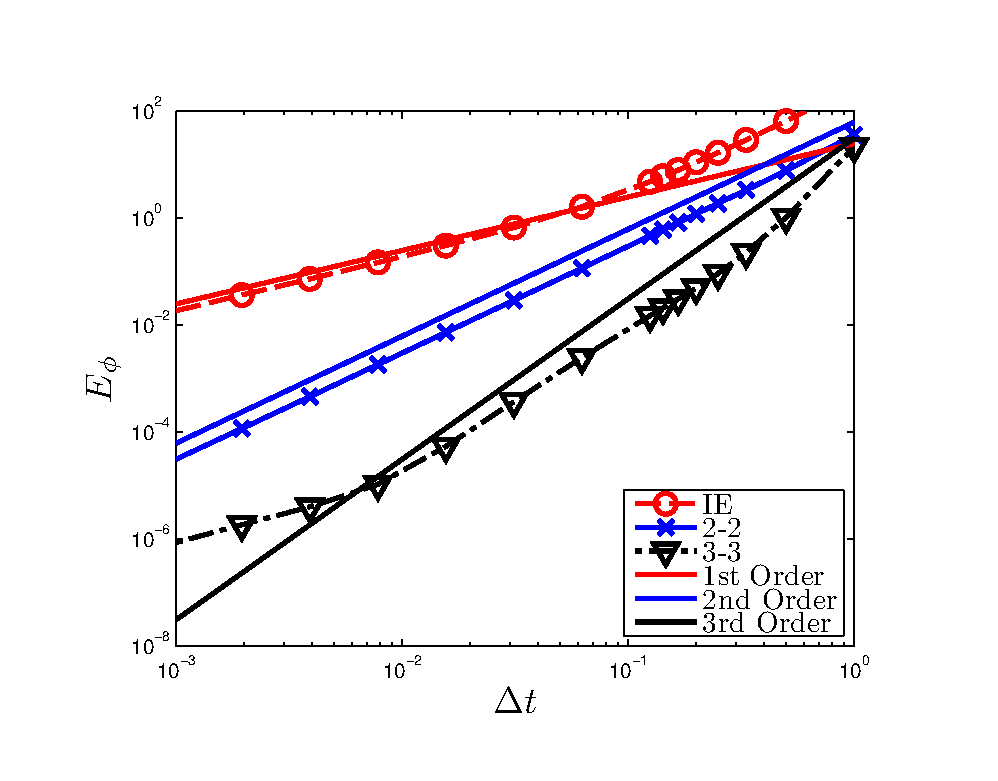
\includegraphics[width=\textwidth,trim=0.25in  0.2in 0.75in 0.5in,clip=true]{../chapter6_grey_radtran/Dissertation_Data/Time_Integrators_Convergence_Phi.pdf}
\end{columns}
\end{frame}


\begin{frame}
\frametitle{Constant Material Properties- MMS1}
\bea
M(\mu_d) &=& \frac{1}{4\pi} \\
F(t) &=& 1+.02t \\
W_I(x) &=& 10 \cos\left( \frac{\pi x}{10} - \frac{\pi}{2} \right) + 15 \\
W_T(x) &=& 25 \cos\left( \frac{\pi x}{10} - \frac{\pi}{2} \right) + 30 \\
C_v &=& 0.1 \\
\sigma_a &=& 100 \\ 
\sigma_s &=& 0.5 \\
t &\in& [0,1] \\
\Delta t &=& 0.01 \\
\eea
Used $S_8$ quadrature, 2-2 SDIRK scheme
\end{frame}

\begin{frame}
\frametitle{TL- MMS1 Results}
TL does not get better applied to a harder problem
\begin{columns}[t]
\column{0.5\textwidth}
\centering
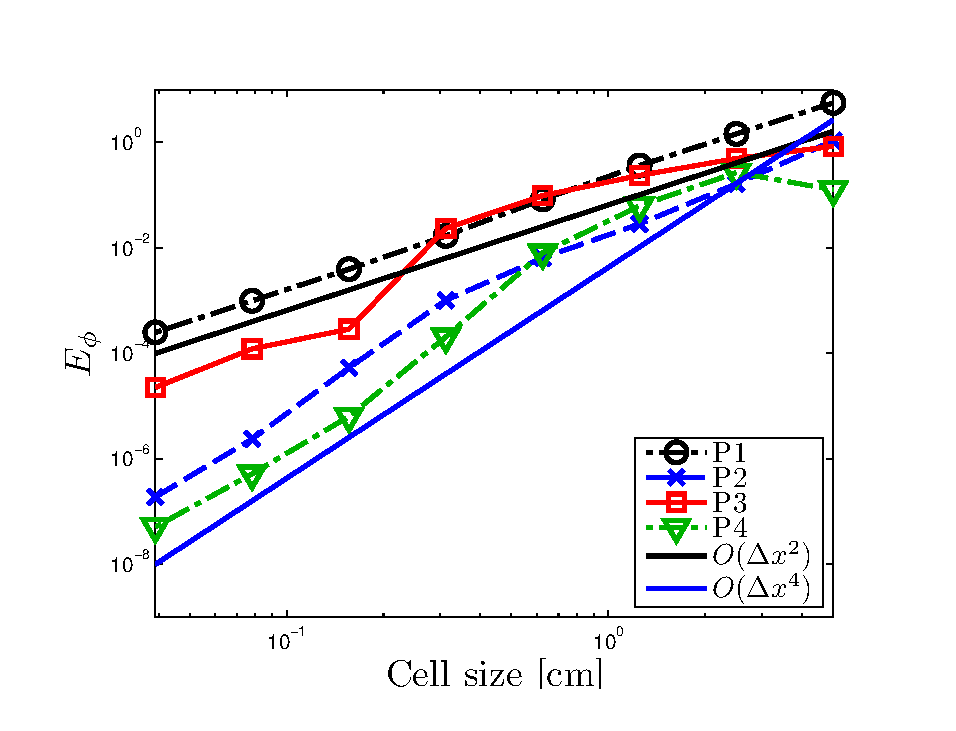
\includegraphics[width=\textwidth,trim=0.25in  0.2in 0.75in 0.5in,clip=true]{../chapter6_grey_radtran/Dissertation_Data/MMS2_TL_phi_L2.pdf}
\column{0.5\textwidth}
\centering
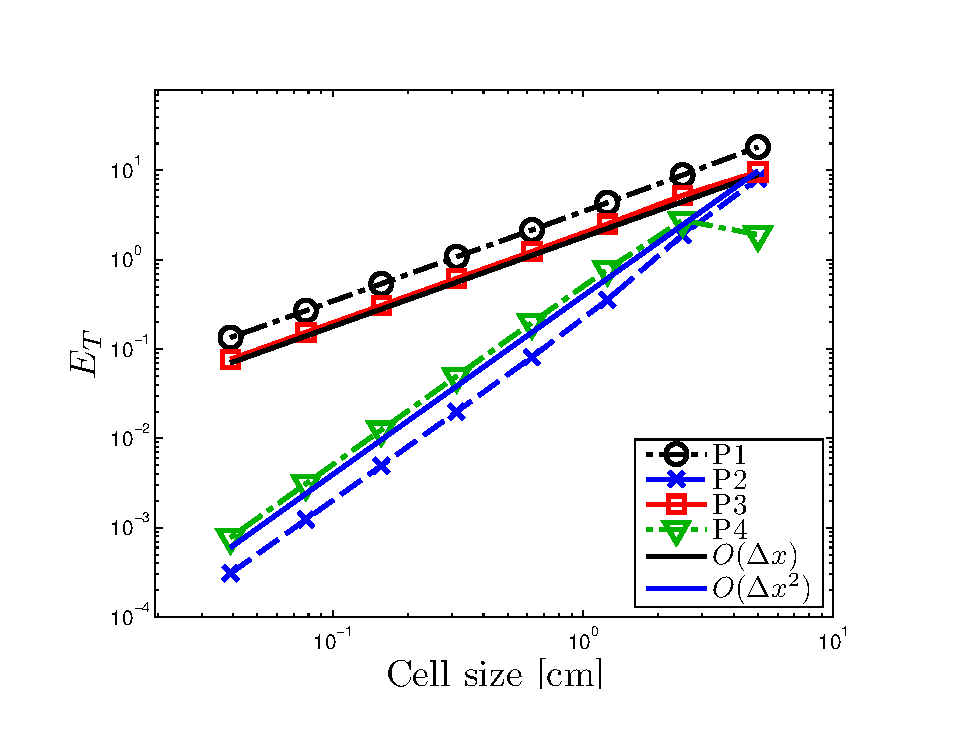
\includegraphics[width=\textwidth,trim=0.25in  0.2in 0.75in 0.5in,clip=true]{../chapter6_grey_radtran/Dissertation_Data/MMS2_TL_temp_L2.pdf}
\end{columns}
\end{frame}

\begin{frame}
\frametitle{SL Lobatto- MMS1 Results}
SL Lobatto loses an order in $T$
\begin{columns}[t]
\column{0.5\textwidth}
\centering
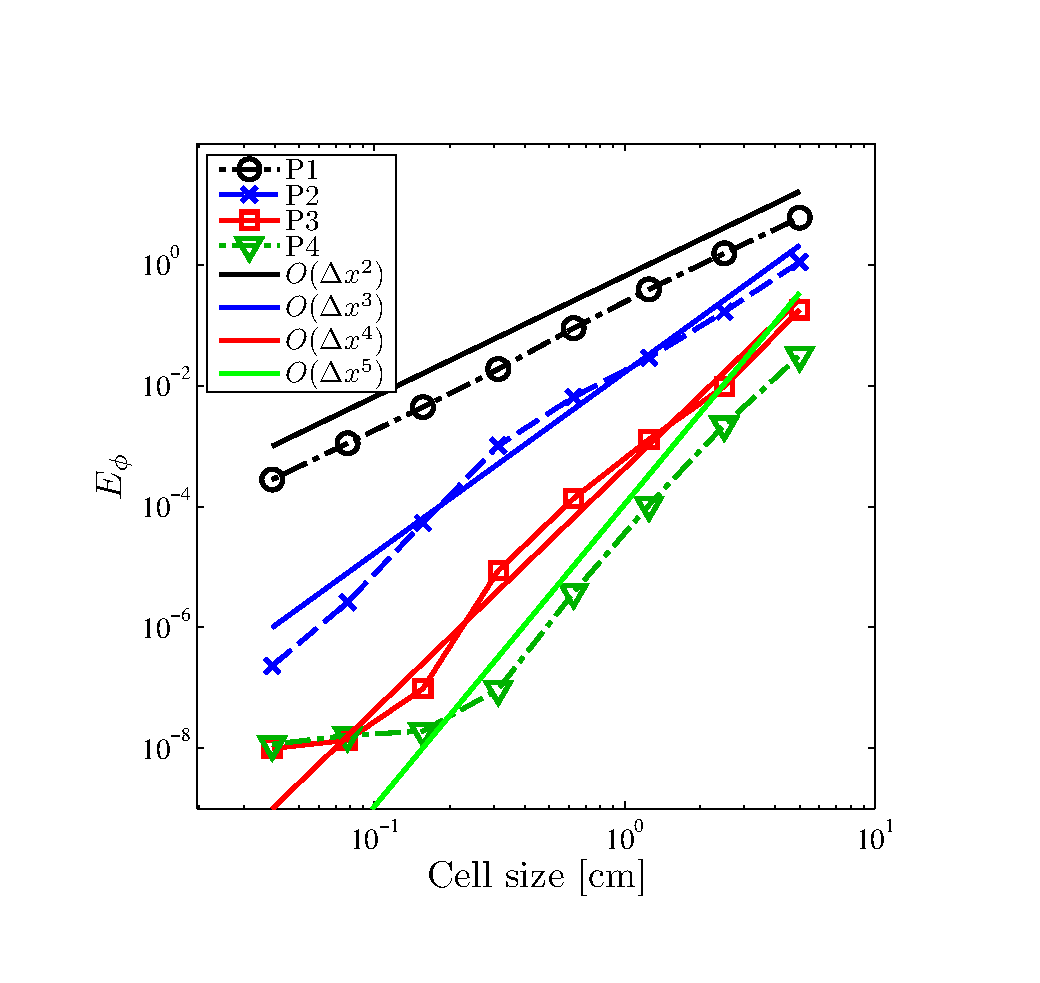
\includegraphics[width=\textwidth,trim=0.25in  0.2in 0.75in 0.5in,clip=true]{../chapter6_grey_radtran/Dissertation_Data/MMS2_SLXS_Lobatto_phi_L2.pdf}
\column{0.5\textwidth}
\centering
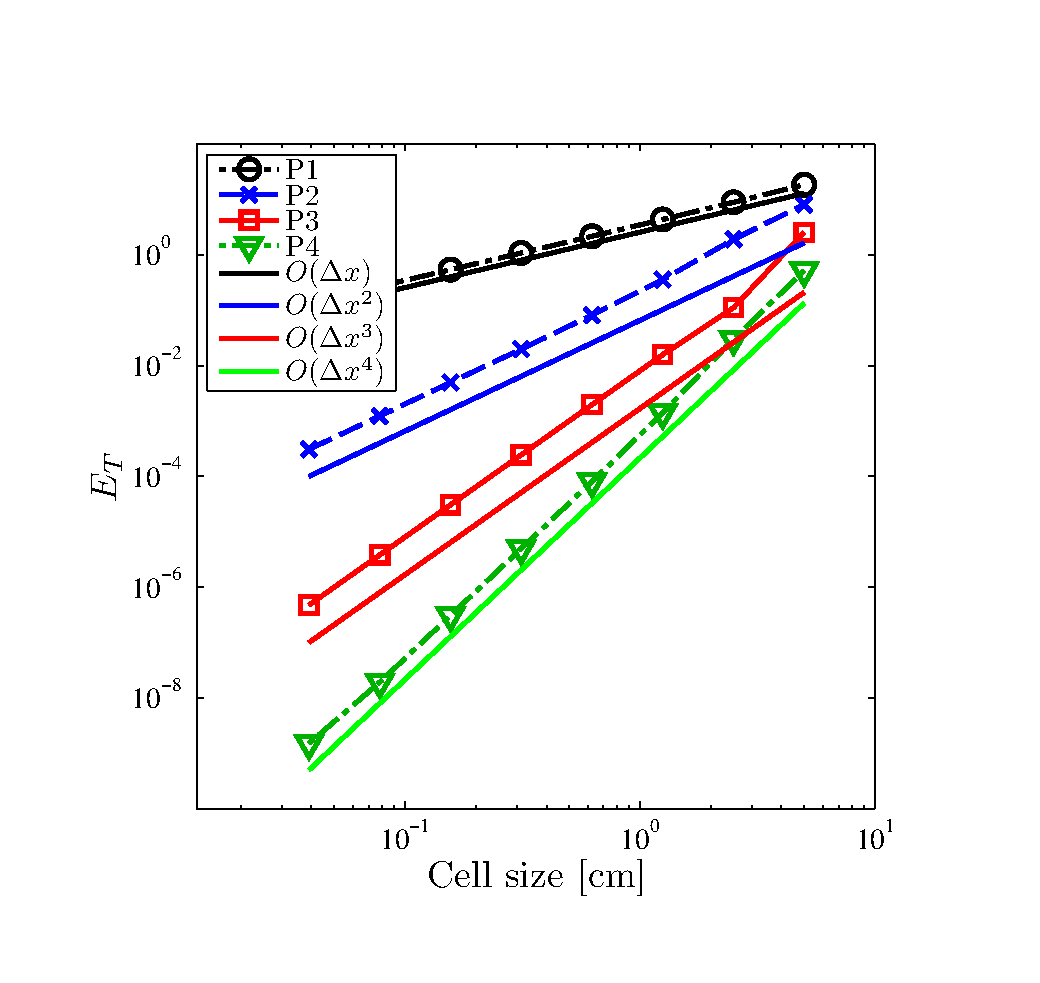
\includegraphics[width=\textwidth,trim=0.25in  0.2in 0.75in 0.5in,clip=true]{../chapter6_grey_radtran/Dissertation_Data/MMS2_SLXS_Lobatto_temp_L2.pdf}
\end{columns}
\end{frame}

\begin{frame}
\frametitle{SL Gauss- MMS1 Results}
SL Gauss picks up an order for $T$?
\begin{columns}[t]
\column{0.5\textwidth}
\centering
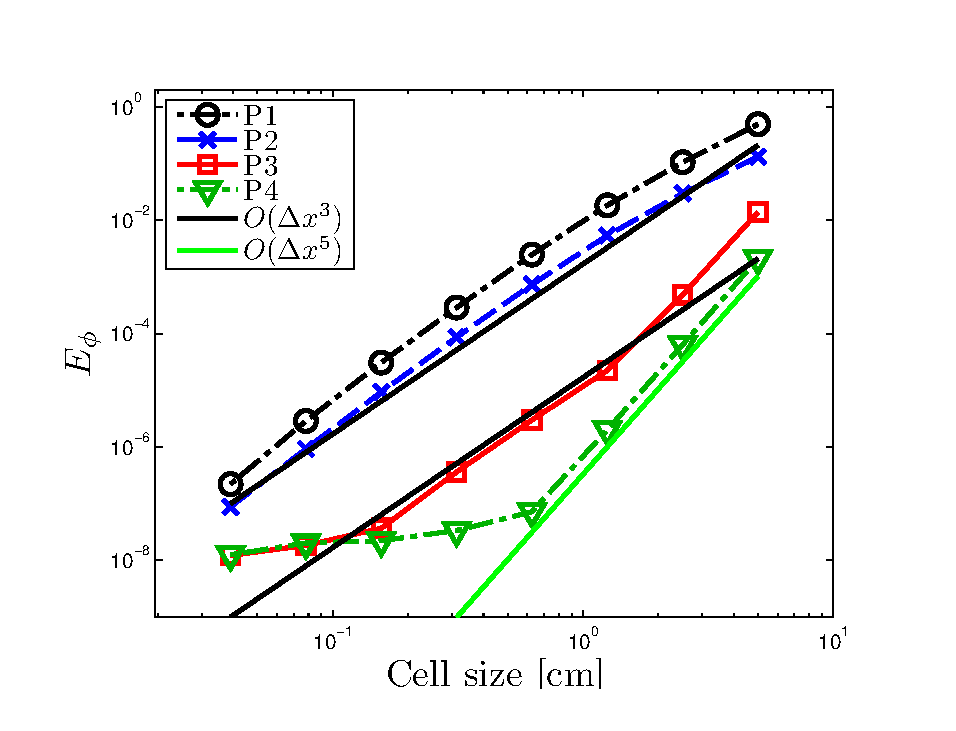
\includegraphics[width=\textwidth,trim=0.25in  0.2in 0.75in 0.5in,clip=true]{../chapter6_grey_radtran/Dissertation_Data/MMS2_SLXS_Gauss_phi_L2.pdf}
\column{0.5\textwidth}
\centering
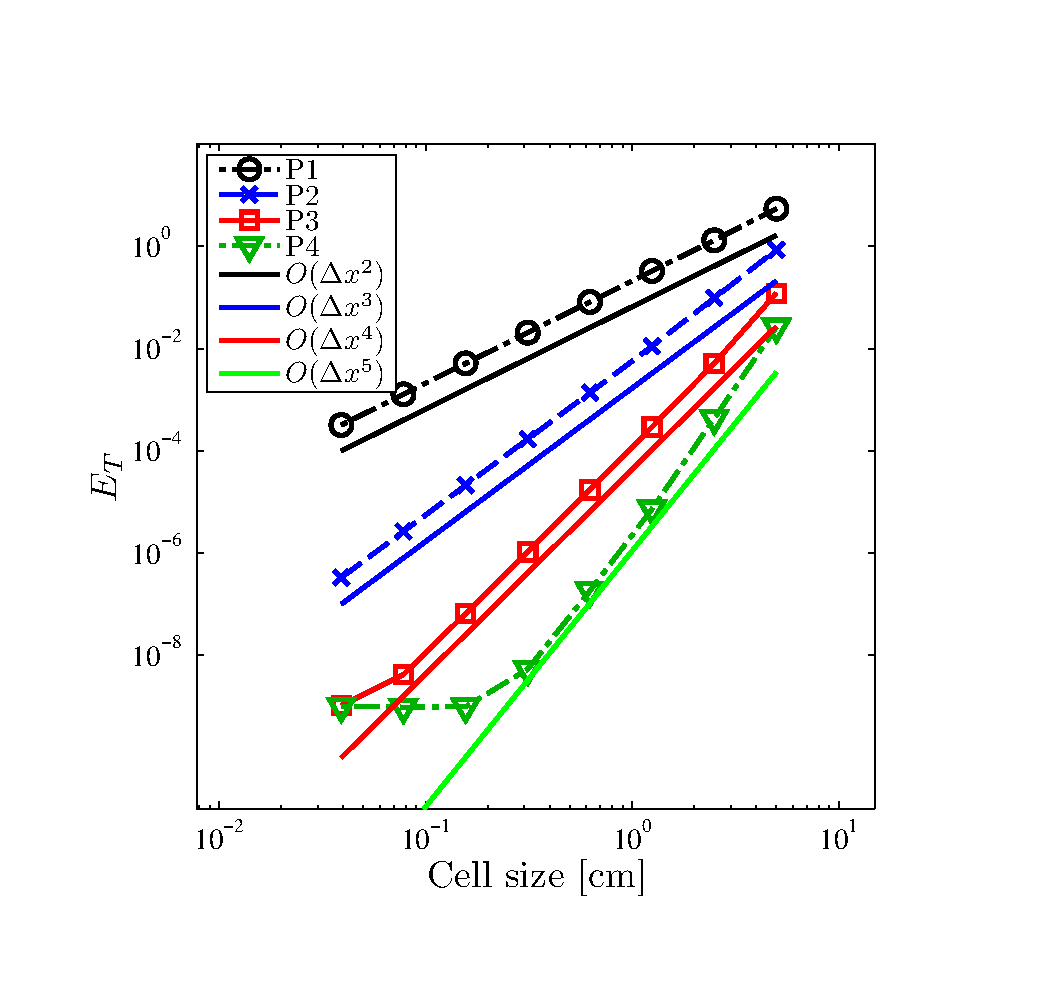
\includegraphics[width=\textwidth,trim=0.25in  0.2in 0.75in 0.5in,clip=true]{../chapter6_grey_radtran/Dissertation_Data/MMS2_SLXS_Gauss_temp_L2.pdf}
\end{columns}
\end{frame}

\begin{frame}
\frametitle{Variable Material Properties- MMS2}
\bea
M(\mu_d) &=& \frac{1}{4\pi} \\
W_I(x) &=& 9 \cos\left( \frac{\pi x}{10} - \frac{\pi}{2} \right) + 3  \\
W_T(x) &=&  5 \cos\left( \frac{\pi x}{10} - \frac{\pi}{2} \right) + 5 \\
F(t) &=&  1 + .02t \\
C_v &=& 0.2 + 0.01 T^3 \\
\sigma_a &=& \frac{10^4}{T^3} \\
\sigma_s &=& 0.5 
\eea
3-3 Alexander, $\Delta t = 10^{-3}$
\end{frame}

\begin{frame}
\frametitle{Must Account for Spatially Varying Material Properties}
SL Gauss, $P\in[1,4]$.  Limited $L^2$ convergence.
\begin{columns}[t]
\column{0.5\textwidth}
\centering
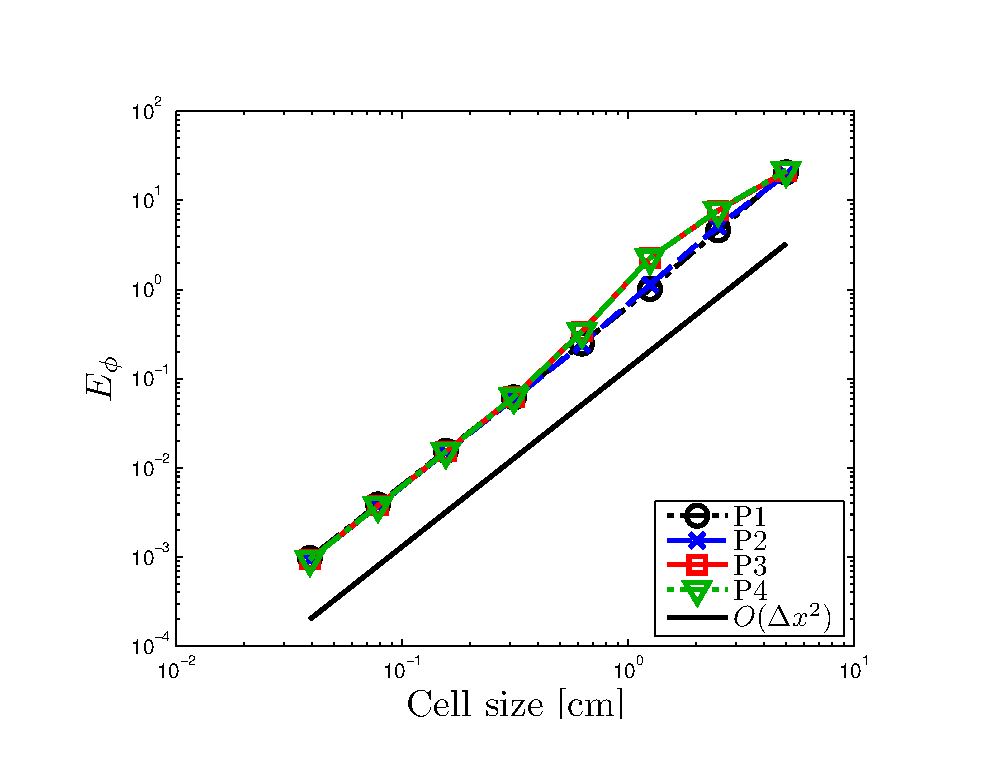
\includegraphics[width=\textwidth,trim=0.25in  0.2in 0.75in 0.5in,clip=true]{../chapter6_grey_radtran/Dissertation_Data/MMS3_Constant_XS_SL_Gauss_phi_L2.pdf}
\column{0.5\textwidth}
\centering
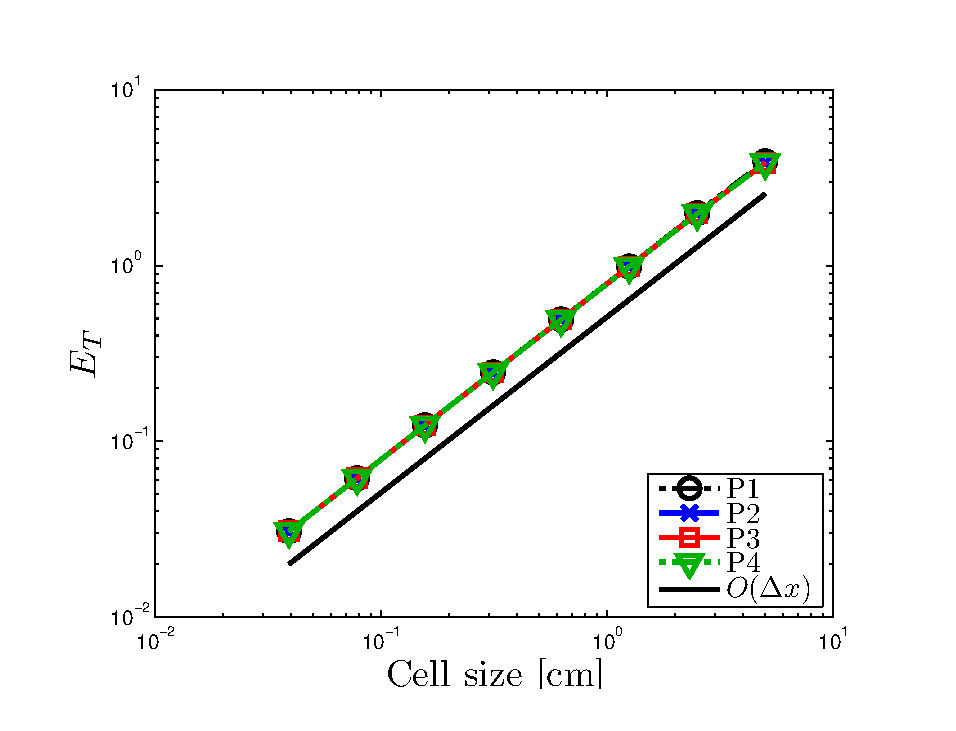
\includegraphics[width=\textwidth,trim=0.25in  0.2in 0.75in 0.5in,clip=true]{../chapter6_grey_radtran/Dissertation_Data/MMS3_Constant_XS_SL_Gauss_temp_L2.pdf}
\end{columns}
\end{frame}

\begin{frame}
\frametitle{Not Lucky This Time}
SL Gauss, $P\in[1,4]$.  High convergence of CXS DFEM for neutronics was problem specific luck/fluke
\begin{columns}[t]
\column{0.5\textwidth}
\centering
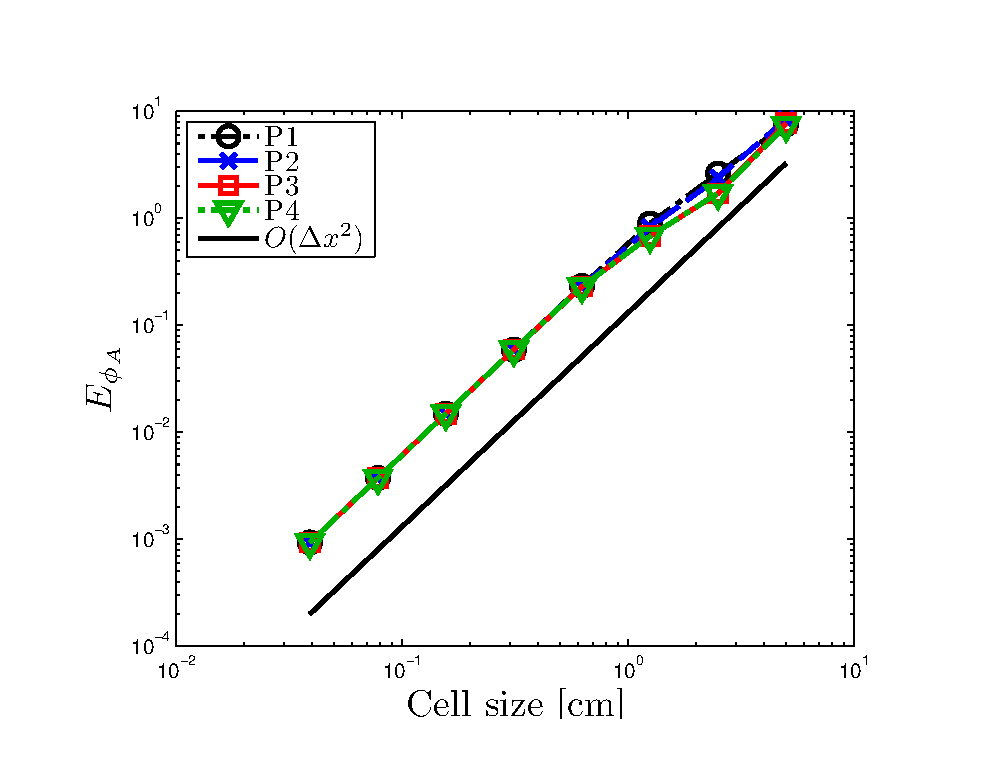
\includegraphics[width=\textwidth,trim=0.25in  0.2in 0.75in 0.5in,clip=true]{../chapter6_grey_radtran/Dissertation_Data/MMS3_Constant_XS_SL_Gauss_phi_A.pdf}
\column{0.5\textwidth}
\centering
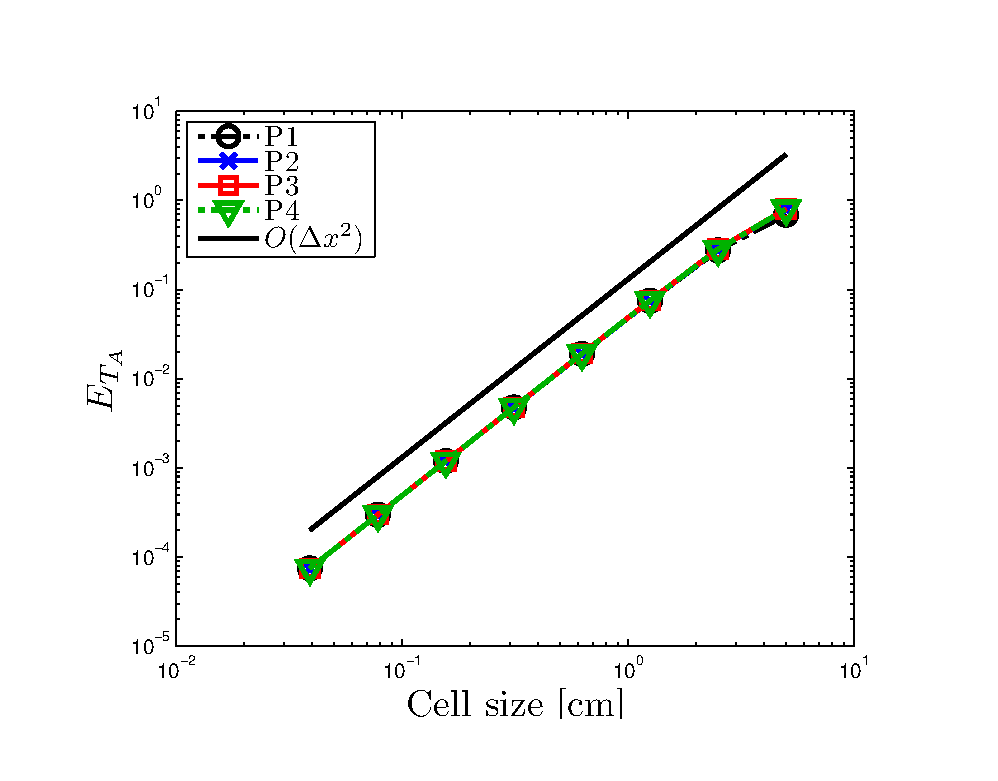
\includegraphics[width=\textwidth,trim=0.25in  0.2in 0.75in 0.5in,clip=true]{../chapter6_grey_radtran/Dissertation_Data/MMS3_Constant_XS_SL_Gauss_temp_A.pdf}
\end{columns}
\end{frame}

\begin{frame}
\frametitle{SLXS $E_{\phi}$ Convergence}
\begin{columns}[t]
\column{0.5\textwidth}
\centering
SLXS Lobatto
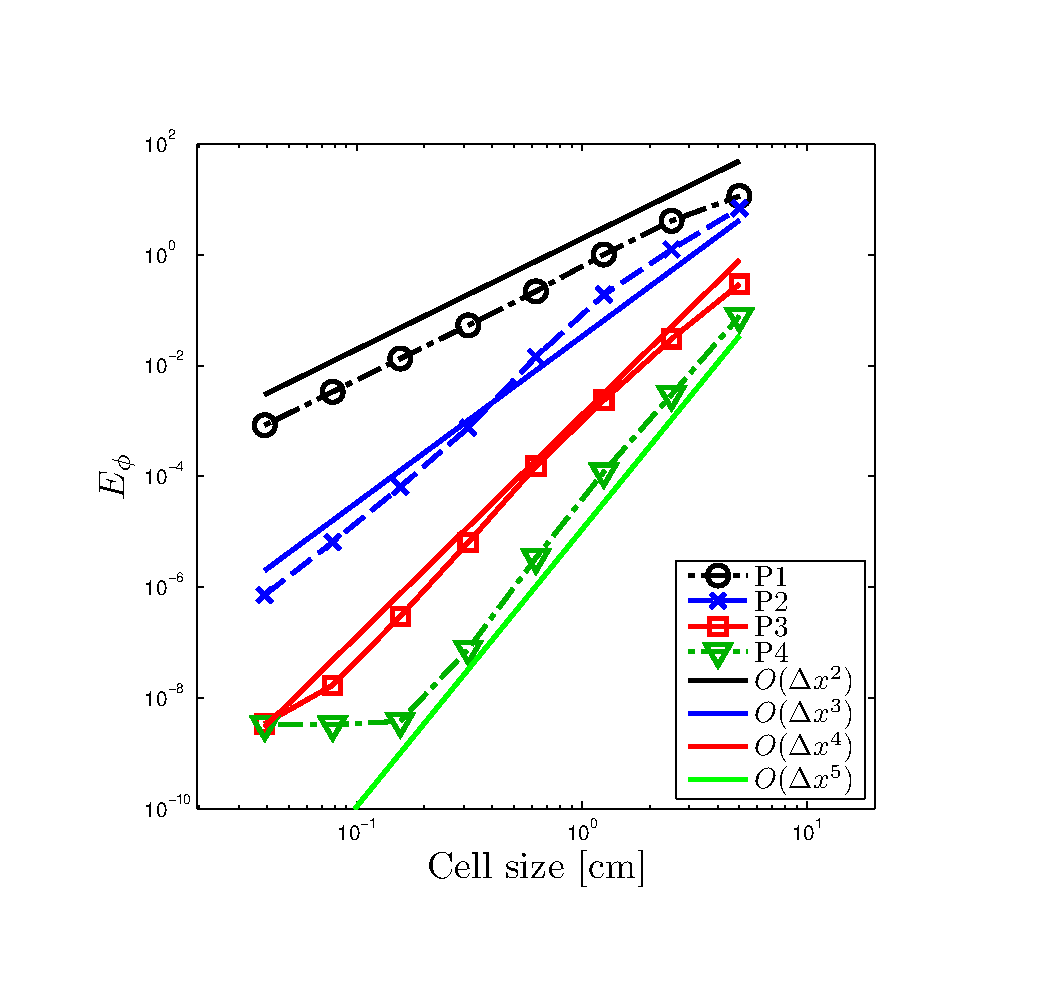
\includegraphics[width=\textwidth,trim=0.25in  0.2in 0.75in 0.5in,clip=true]{../chapter6_grey_radtran/Dissertation_Data/MMS3_SLXS_Lobatto_phi_L2.pdf}
\\
$\propto P+1$
\column{0.5\textwidth}
\centering
SLXS Gauss
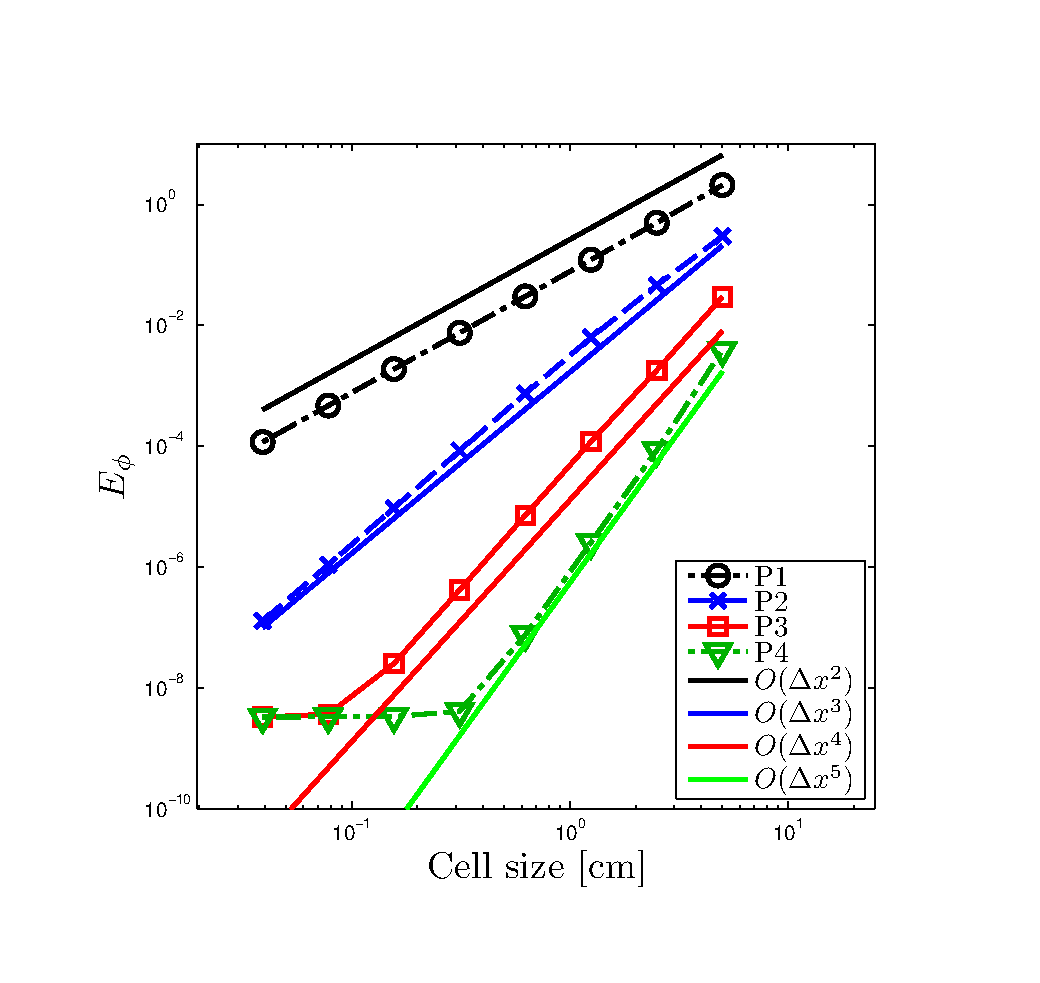
\includegraphics[width=\textwidth,trim=0.25in  0.2in 0.75in 0.5in,clip=true]{../chapter6_grey_radtran/Dissertation_Data/MMS3_SLXS_Gauss_phi_L2.pdf}
\\
$\propto P+1$
\end{columns}
\end{frame}

\begin{frame}
\frametitle{SLXS $E_T$ Convergence}
\begin{columns}[t]
\column{0.5\textwidth}
\centering
SLXS Lobatto
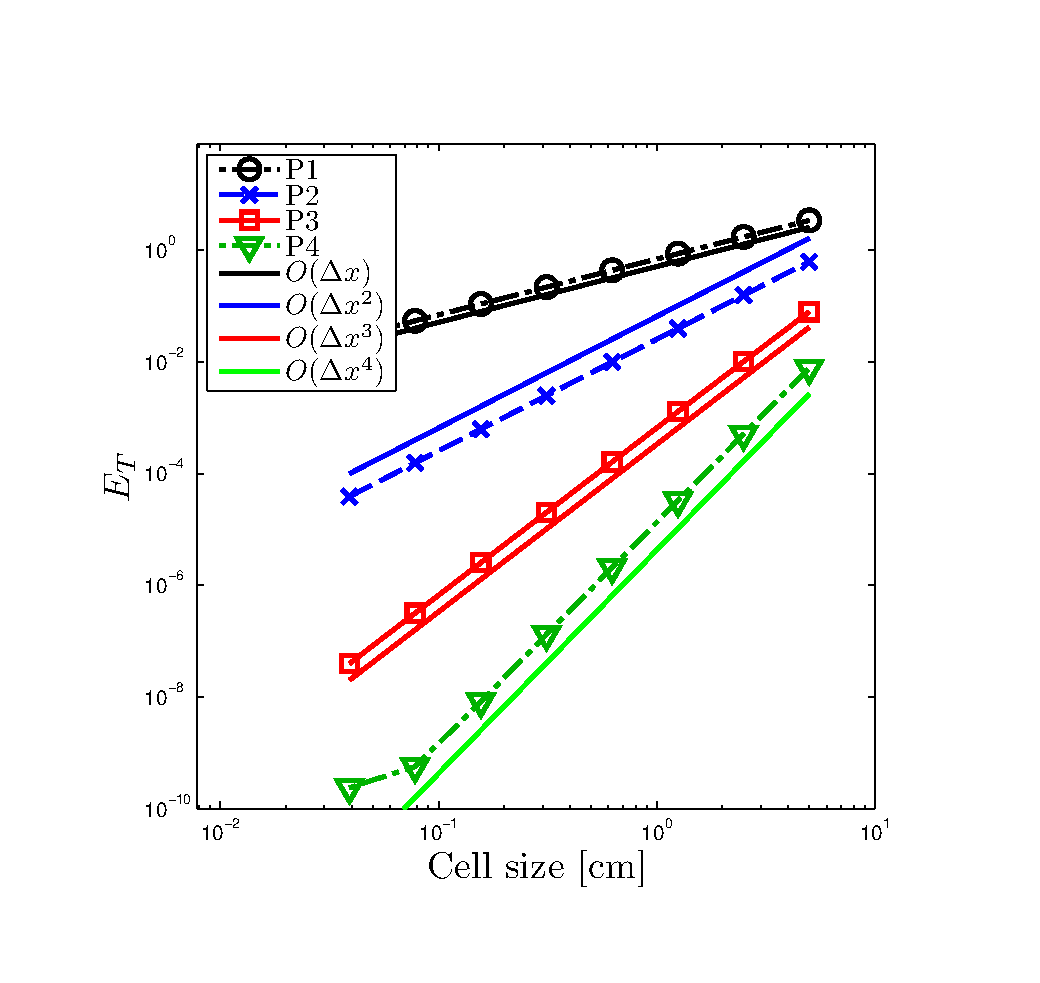
\includegraphics[width=\textwidth,trim=0.25in  0.2in 0.75in 0.5in,clip=true]{../chapter6_grey_radtran/Dissertation_Data/MMS3_SLXS_Lobatto_temp_L2.pdf}
\\
$\propto P$
\column{0.5\textwidth}
\centering
SLXS Gauss
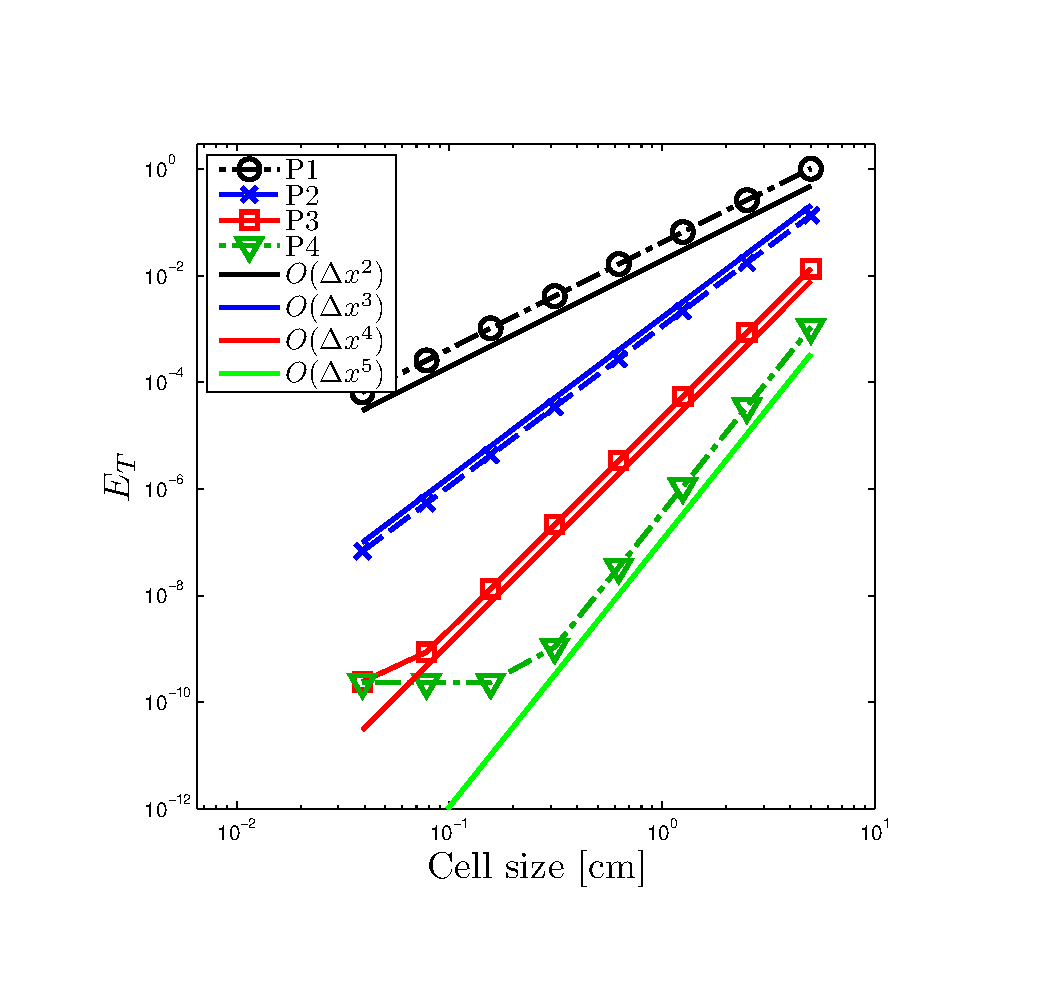
\includegraphics[width=\textwidth,trim=0.25in  0.2in 0.75in 0.5in,clip=true]{../chapter6_grey_radtran/Dissertation_Data/MMS3_SLXS_Gauss_temp_L2.pdf}
\\
$\propto P+1$
\end{columns}
\end{frame}

\begin{frame}
\frametitle{Steady-state problem}
\bea
M(\mu_d) &=& \frac{1}{4\pi} \\
W_I(x) &=& 19 \cos\left( \frac{\pi x}{2} \right) + 20 \pec \\
W_T(x) &=&  15 \cos\left( \frac{\pi x}{2}  \right) + 20 \pec \\
F(t) &=&  10 \\
C_v &=& 0.1 + 0.2 T^2 \\
\sigma_a &=& \frac{5}{T^2} \\
\sigma_s &=& 0.01 
\eea

\end{frame}

\begin{frame}
\frametitle{SLXS Lobatto $L^2$ Convergence}
\begin{columns}[t]
\column{0.5\textwidth}
\centering
$E_{\phi}$
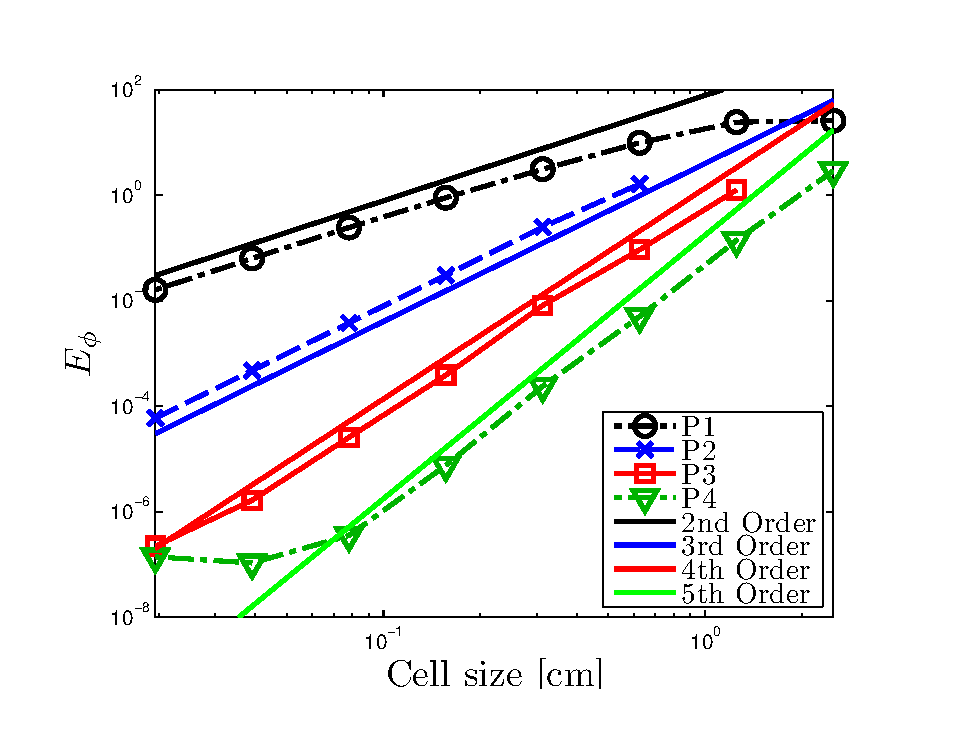
\includegraphics[width=\textwidth,trim=0.25in  0.2in 0.75in 0.5in,clip=true]{../chapter6_grey_radtran/Dissertation_Data/Constant_Time_SLXS_Lobatto_phi_L2.pdf}
\\
$\propto P+1$
\column{0.5\textwidth}
\centering
$E_{T}$
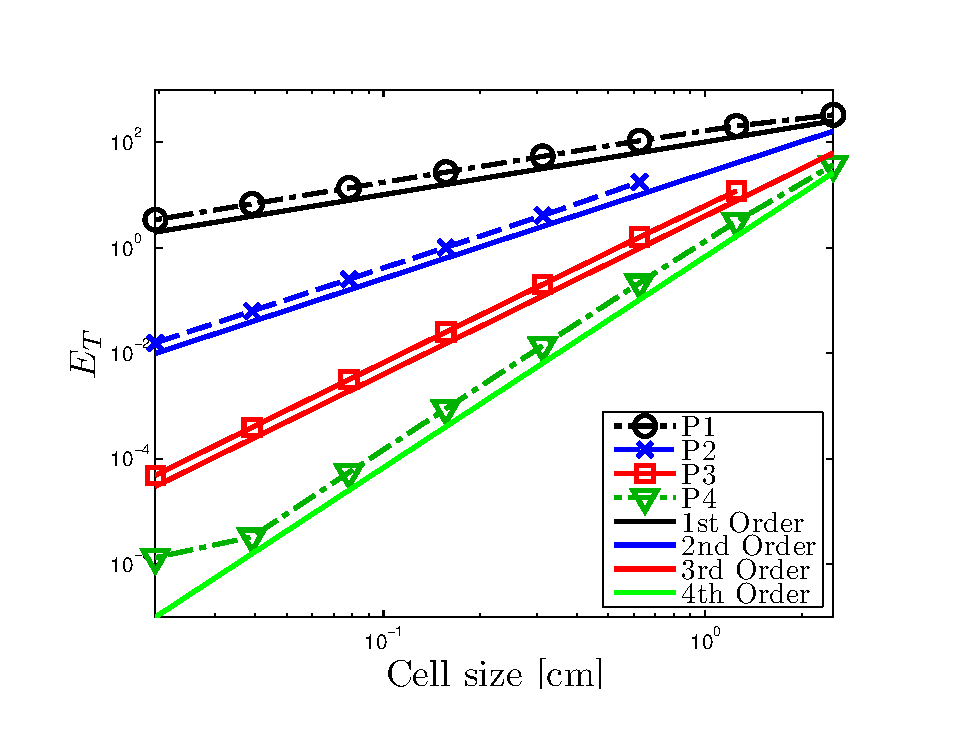
\includegraphics[width=\textwidth,trim=0.25in  0.2in 0.75in 0.5in,clip=true]{../chapter6_grey_radtran/Dissertation_Data/Constant_Time_SLXS_Lobatto_temp_L2.pdf}
\\
$\propto P$
\end{columns}
\centering
No surprises
\end{frame}

\begin{frame}
\frametitle{SLXS Gauss $L^2$ Convergence}
\begin{columns}[t]
\column{0.5\textwidth}
\centering
$E_{\phi}$
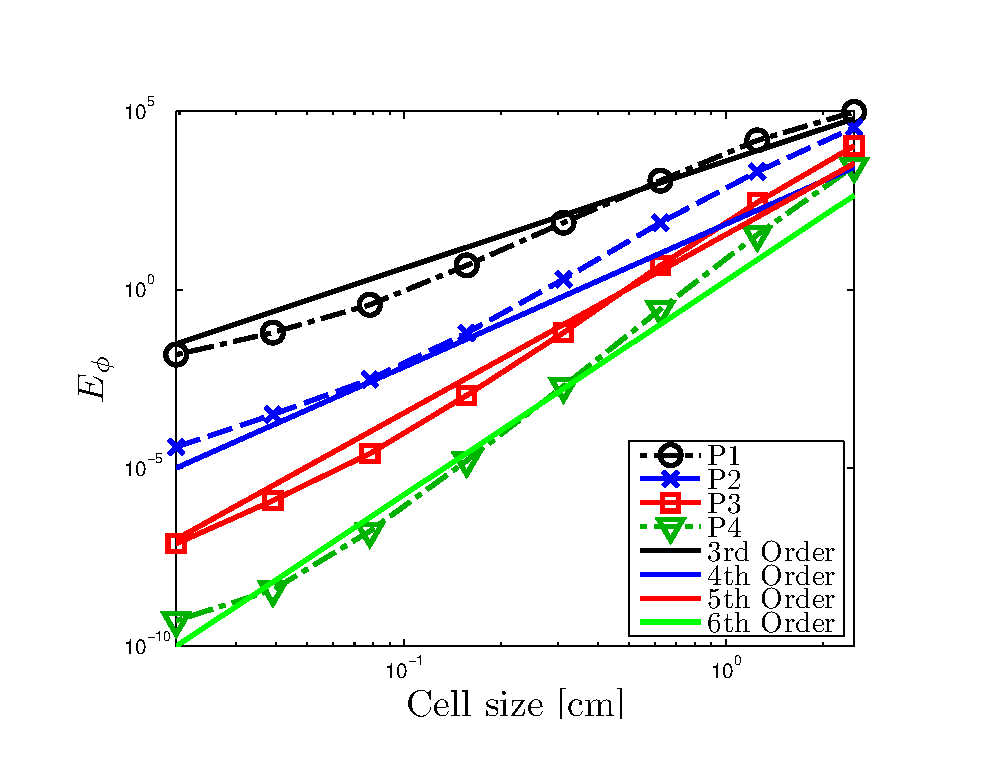
\includegraphics[width=\textwidth,trim=0.25in  0.2in 0.75in 0.5in,clip=true]{../chapter6_grey_radtran/Dissertation_Data/Constant_Time_SLXS_Gauss_phi_L2.pdf}
\\
$\propto P+2$
\column{0.5\textwidth}
\centering
$E_{T}$
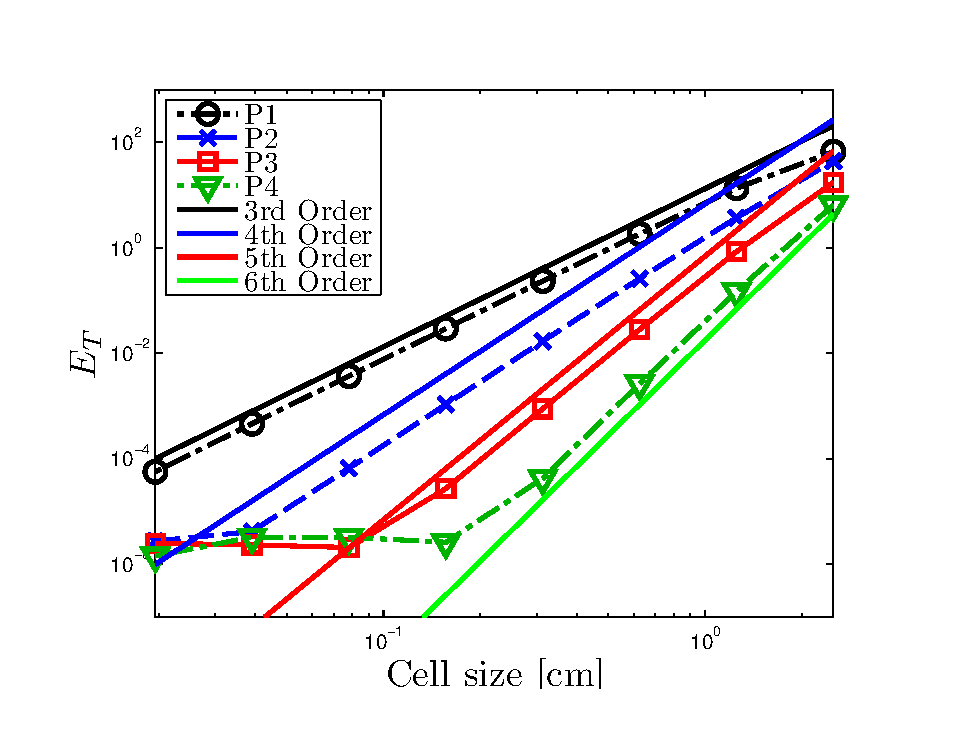
\includegraphics[width=\textwidth,trim=0.25in  0.2in 0.75in 0.5in,clip=true]{../chapter6_grey_radtran/Dissertation_Data/Constant_Time_SLXS_Gauss_temp_L2.pdf}
\\
$\propto P+1$
\end{columns}
\centering
\vspace{0.2in}
Where did the extra order in $E_{\phi}$ come from?
\end{frame}

\begin{frame}
\frametitle{$E_{\phi_A}$ Convergence}
\begin{columns}[t]
\column{0.5\textwidth}
\centering
SLXS Lobatto
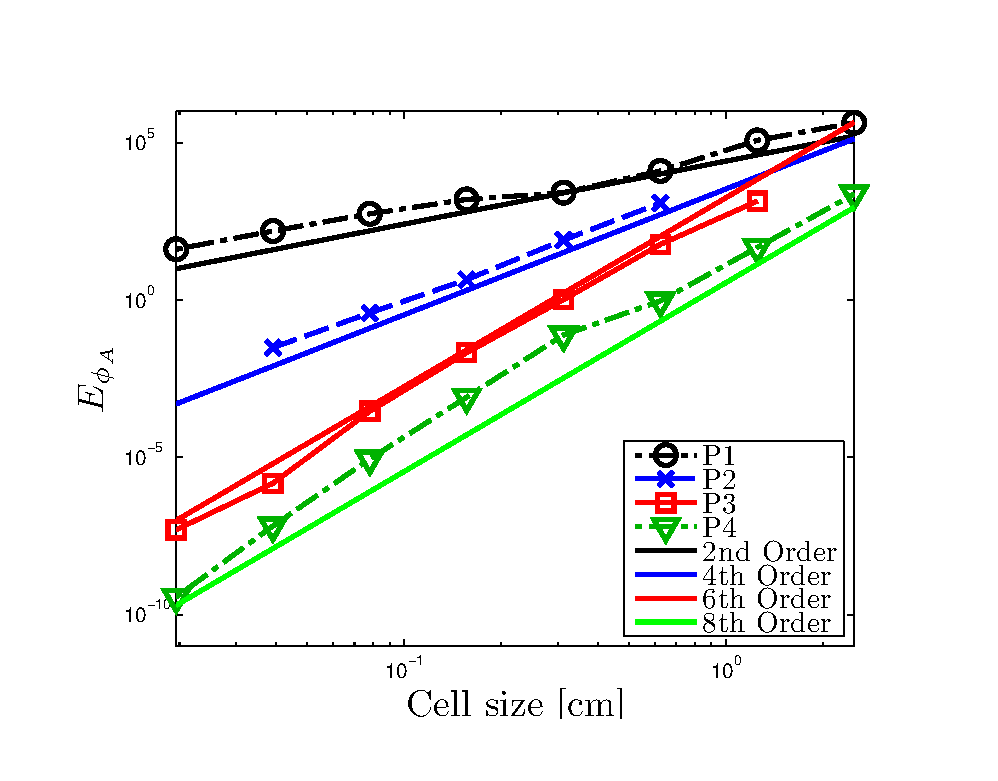
\includegraphics[width=\textwidth,trim=0.25in  0.2in 0.75in 0.5in,clip=true]{../chapter6_grey_radtran/Dissertation_Data/Constant_Time_SLXS_Lobatto_phi_A.pdf}
\\
TRT $E_{\phi_A}\propto 2P$
\\
Neutronics $E_{\psi_A} \propto 2P$
\column{0.5\textwidth}
\centering
SLXS Gauss
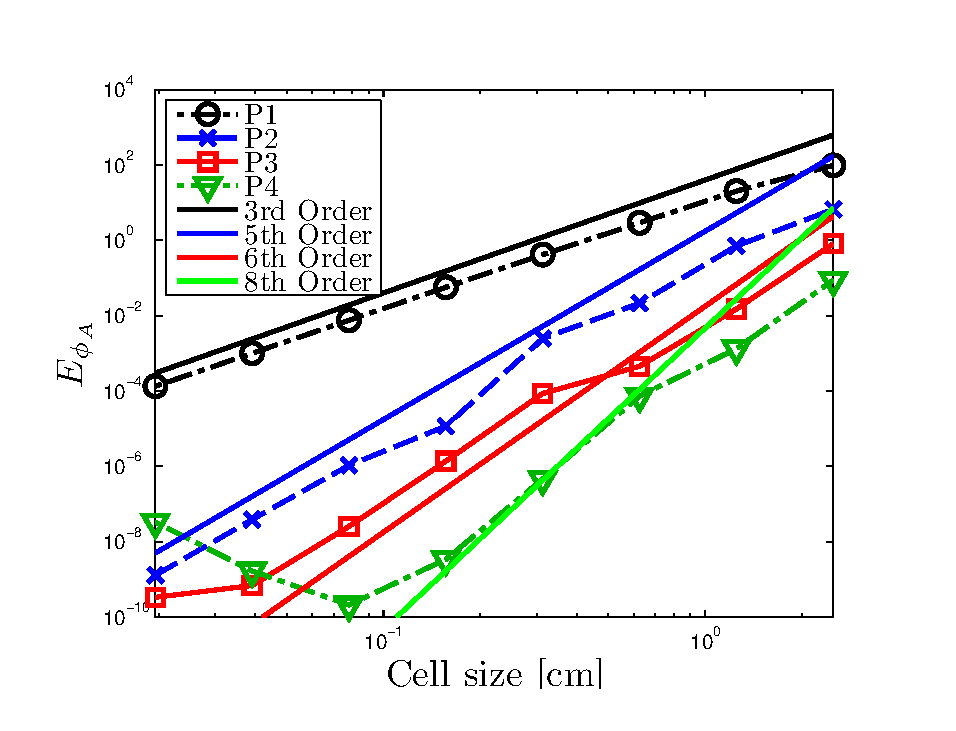
\includegraphics[width=\textwidth,trim=0.25in  0.2in 0.75in 0.5in,clip=true]{../chapter6_grey_radtran/Dissertation_Data/Constant_Time_SLXS_Gauss_phi_A.pdf}
\\ 
TRT $E_{\phi_A} < 2P+2 $
\\
Neutronics $E_{\psi_A} \propto 2P+1$
\end{columns}
\centering
\end{frame}

\begin{frame}
\frametitle{$E_{T_A}$ Convergence}
\begin{columns}[t]
\column{0.5\textwidth}
\centering
SLXS Lobatto
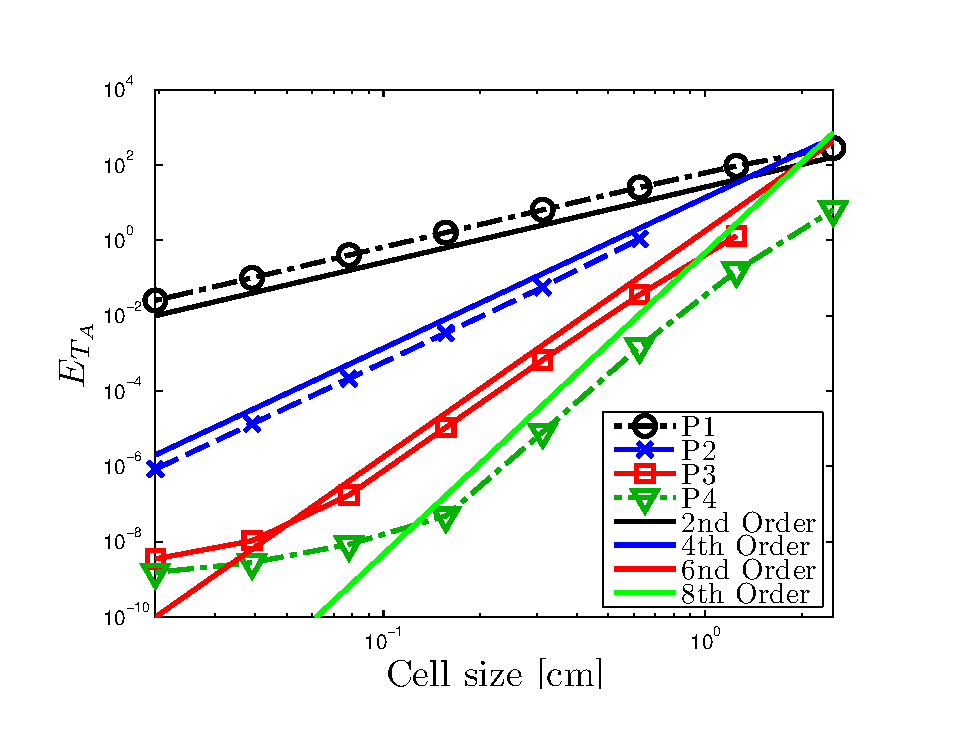
\includegraphics[width=\textwidth,trim=0.25in  0.2in 0.75in 0.5in,clip=true]{../chapter6_grey_radtran/Dissertation_Data/Constant_Time_SLXS_Lobatto_temp_A.pdf}
\\
TRT $E_{T_A}\propto 2P$
\\
Neutronics $E_{\psi_A} \propto 2P$
\column{0.5\textwidth}
\centering
SLXS Gauss
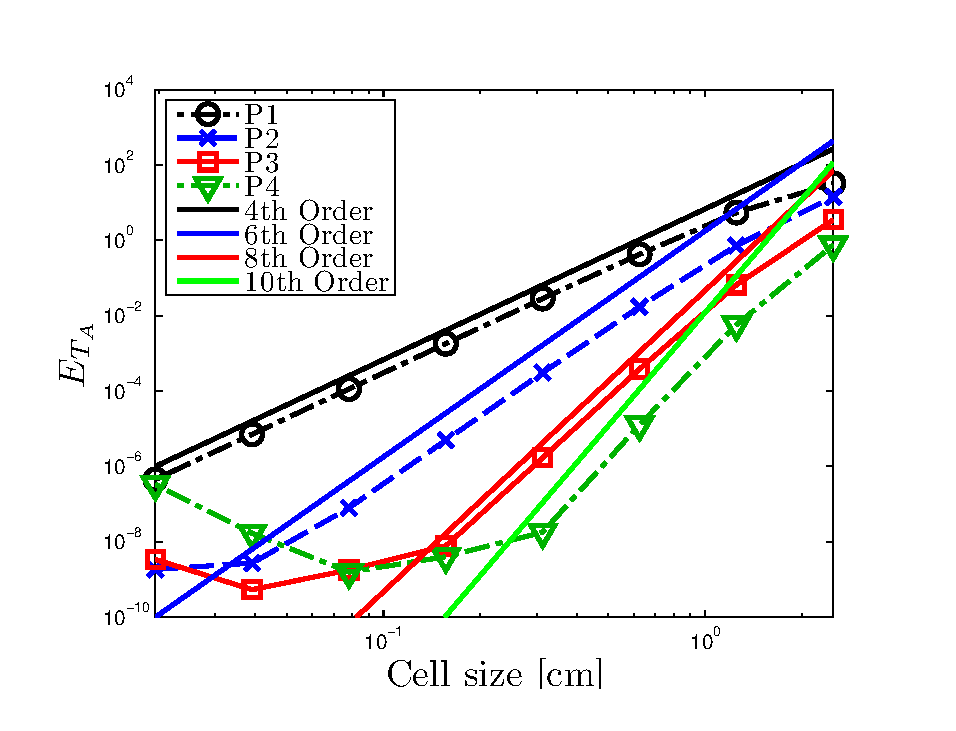
\includegraphics[width=\textwidth,trim=0.25in  0.2in 0.75in 0.5in,clip=true]{../chapter6_grey_radtran/Dissertation_Data/Constant_Time_SLXS_Gauss_temp_A.pdf}
\\
TRT $E_{T_A} \propto 2P+2 $
\\
 Neutronics $E_{\psi_A} \propto 2P+1$
\end{columns}
\centering
\end{frame}


\section{Marshak Wave}
\subsection{Marhsak Wave Blading}
\begin{frame}
\frametitle{Marshak Wave Problem}
Unit current incident intensity on left face.  Vacuum right boundary condition.  Initially cold slab.  No analytic solution.
\bea
a&=&c=C_v = 1 \\
x&\in&[0,1] \\
t&\in&[0,1]  \\
T_0^4& =& 1E-5 \\
\sigma_s &=& 0 \\
\sigma_a &=& \frac{1}{T^3}
\eea
\end{frame}

\begin{frame}
\frametitle{Blading with Cell-Wise Constant Assumption}
Linear TL, volumetric average opacity
\begin{columns}[t]
\column{0.5\textwidth}
\centering
Radiation energy density
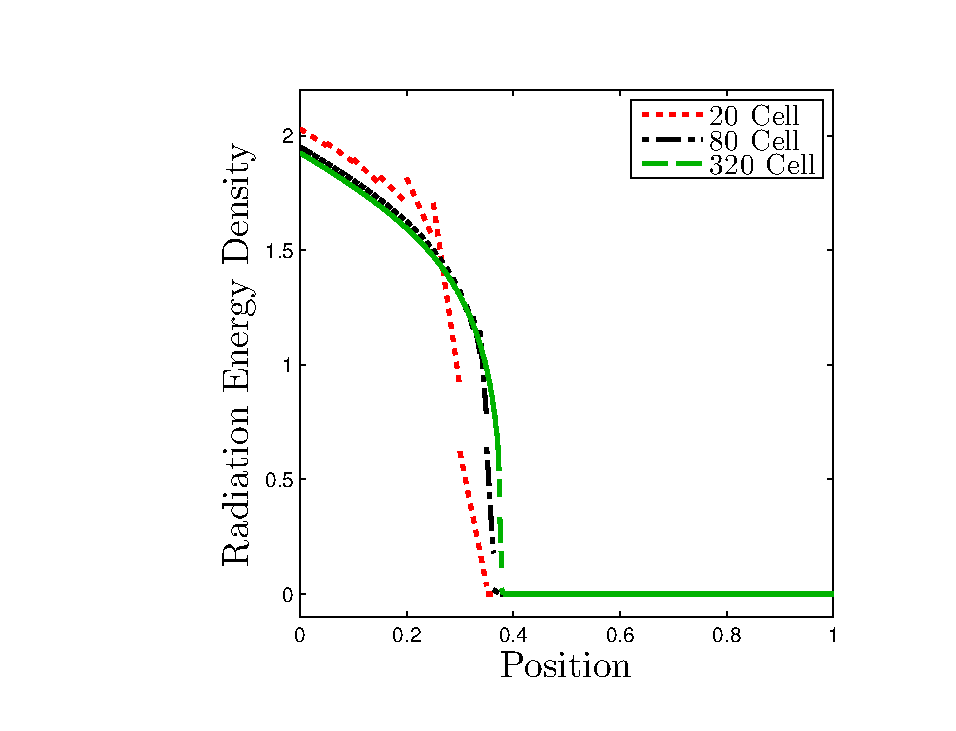
\includegraphics[width=\textwidth,trim=1.2in  0.2in 0.75in 0.5in,clip=true]{../chapter6_grey_radtran/Dissertation_Data/Blading_Radiation_Full_MultiCell.pdf}
\column{0.5\textwidth}
\centering
Material temperature
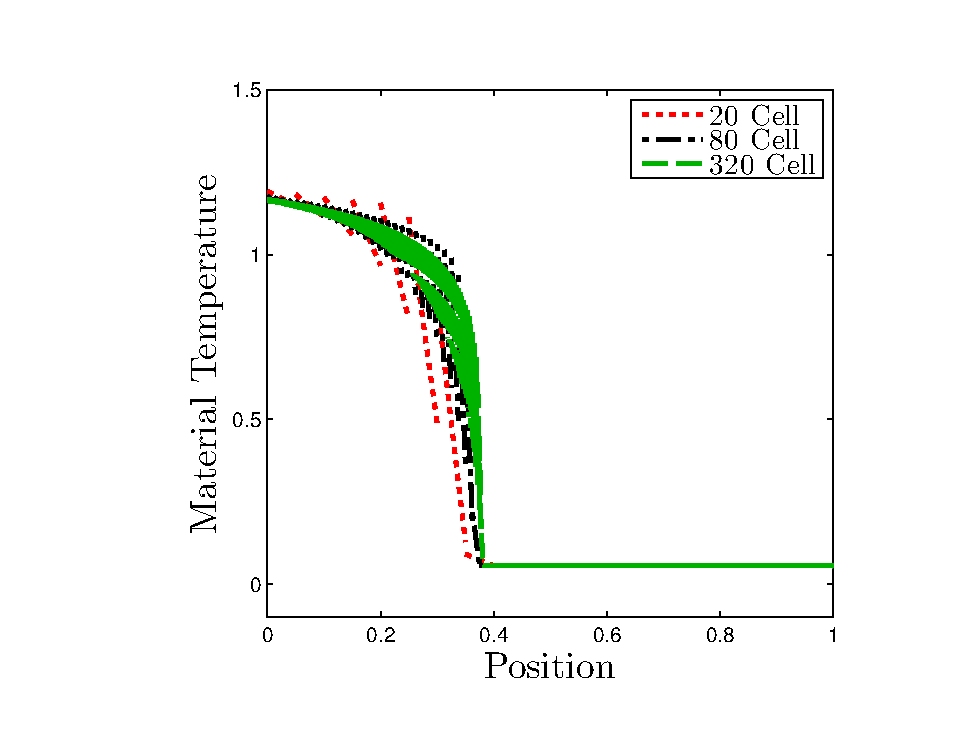
\includegraphics[width=\textwidth,trim=1.2in  0.2in 0.75in 0.5in,clip=true]{../chapter6_grey_radtran/Dissertation_Data/Blading_Temperature_Full_MultiCell.pdf}
\end{columns}
\end{frame}

\begin{frame}
\frametitle{SLXS Treatment}
Linear SLXS Lobatto
\begin{columns}[t]
\column{0.5\textwidth}
\centering
Radiation energy density
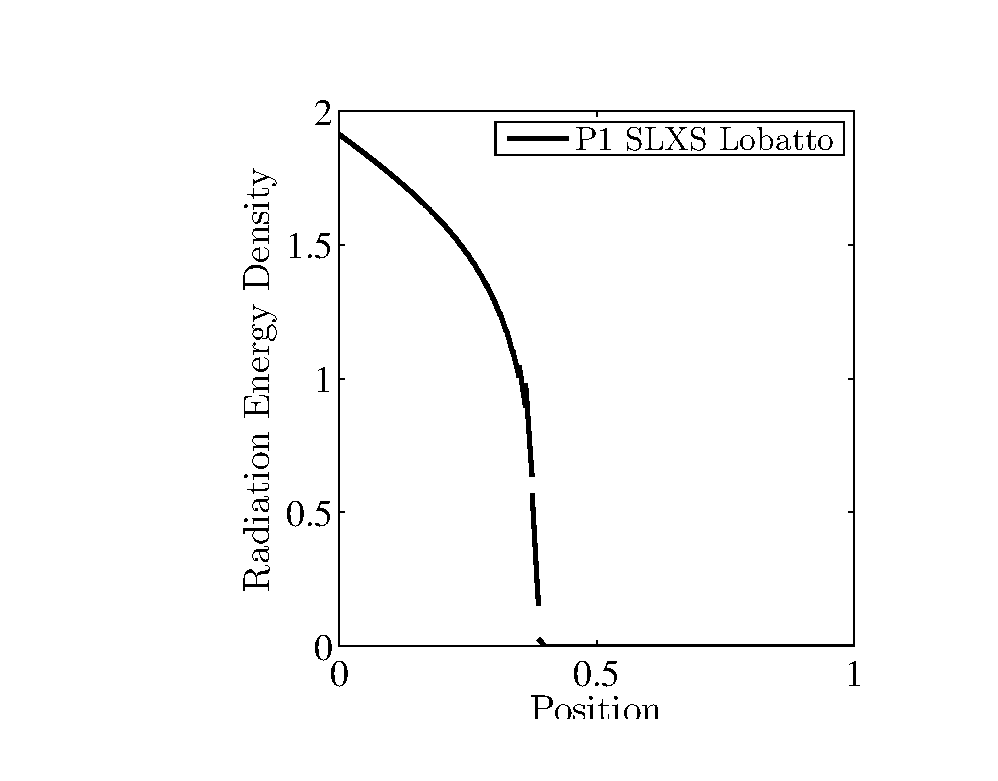
\includegraphics[width=\textwidth,trim=1.2in  0.2in 0.75in 0.5in,clip=true]{../chapter6_grey_radtran/Dissertation_Data/SLXS_Lobatto_80_Cells_Radiation.pdf}
\column{0.5\textwidth}
\centering
Material temperature
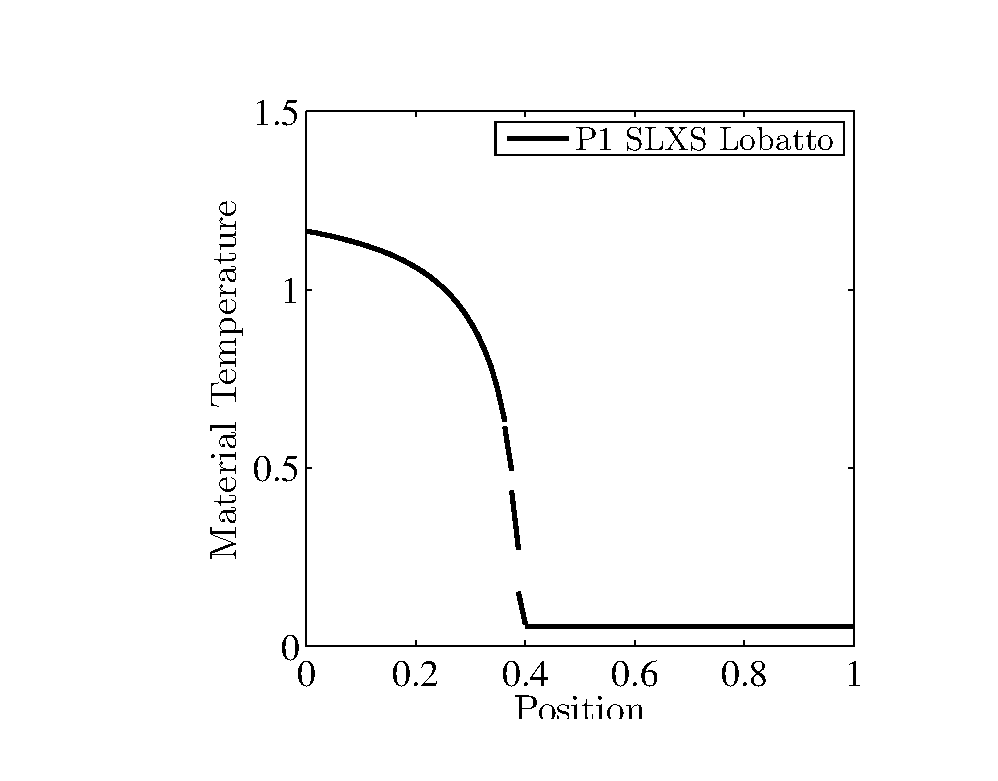
\includegraphics[width=\textwidth,trim=1.2in  0.2in 0.75in 0.5in,clip=true]{../chapter6_grey_radtran/Dissertation_Data/SLXS_Lobatto_80_Cells_Temperature.pdf}
\end{columns}
\end{frame}

\begin{frame}
\frametitle{Time Resolution Cannot Be Neglected}
\centering
Quartic SLXS Lobatto, 1280 mesh cells, 2-2 SDIRK, $\Delta t = 0.01$
\\
\vspace{0.1in}
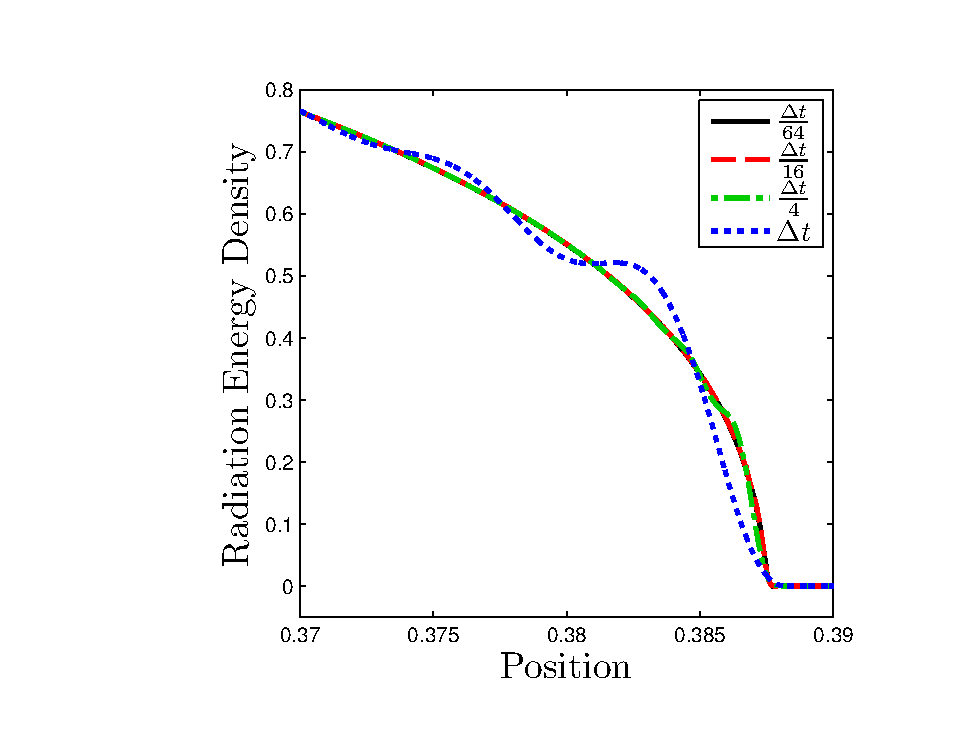
\includegraphics[width=0.9\textheight,trim=1.0in  0.2in 0.5in 0.5in,clip=true]{../chapter6_grey_radtran/Dissertation_Data/Time_Refinement_Zoom_Radiation.pdf}
\end{frame}


\begin{frame}
\frametitle{Extreme Zoom of $S_2$ Radiation Energy Density}
\centering
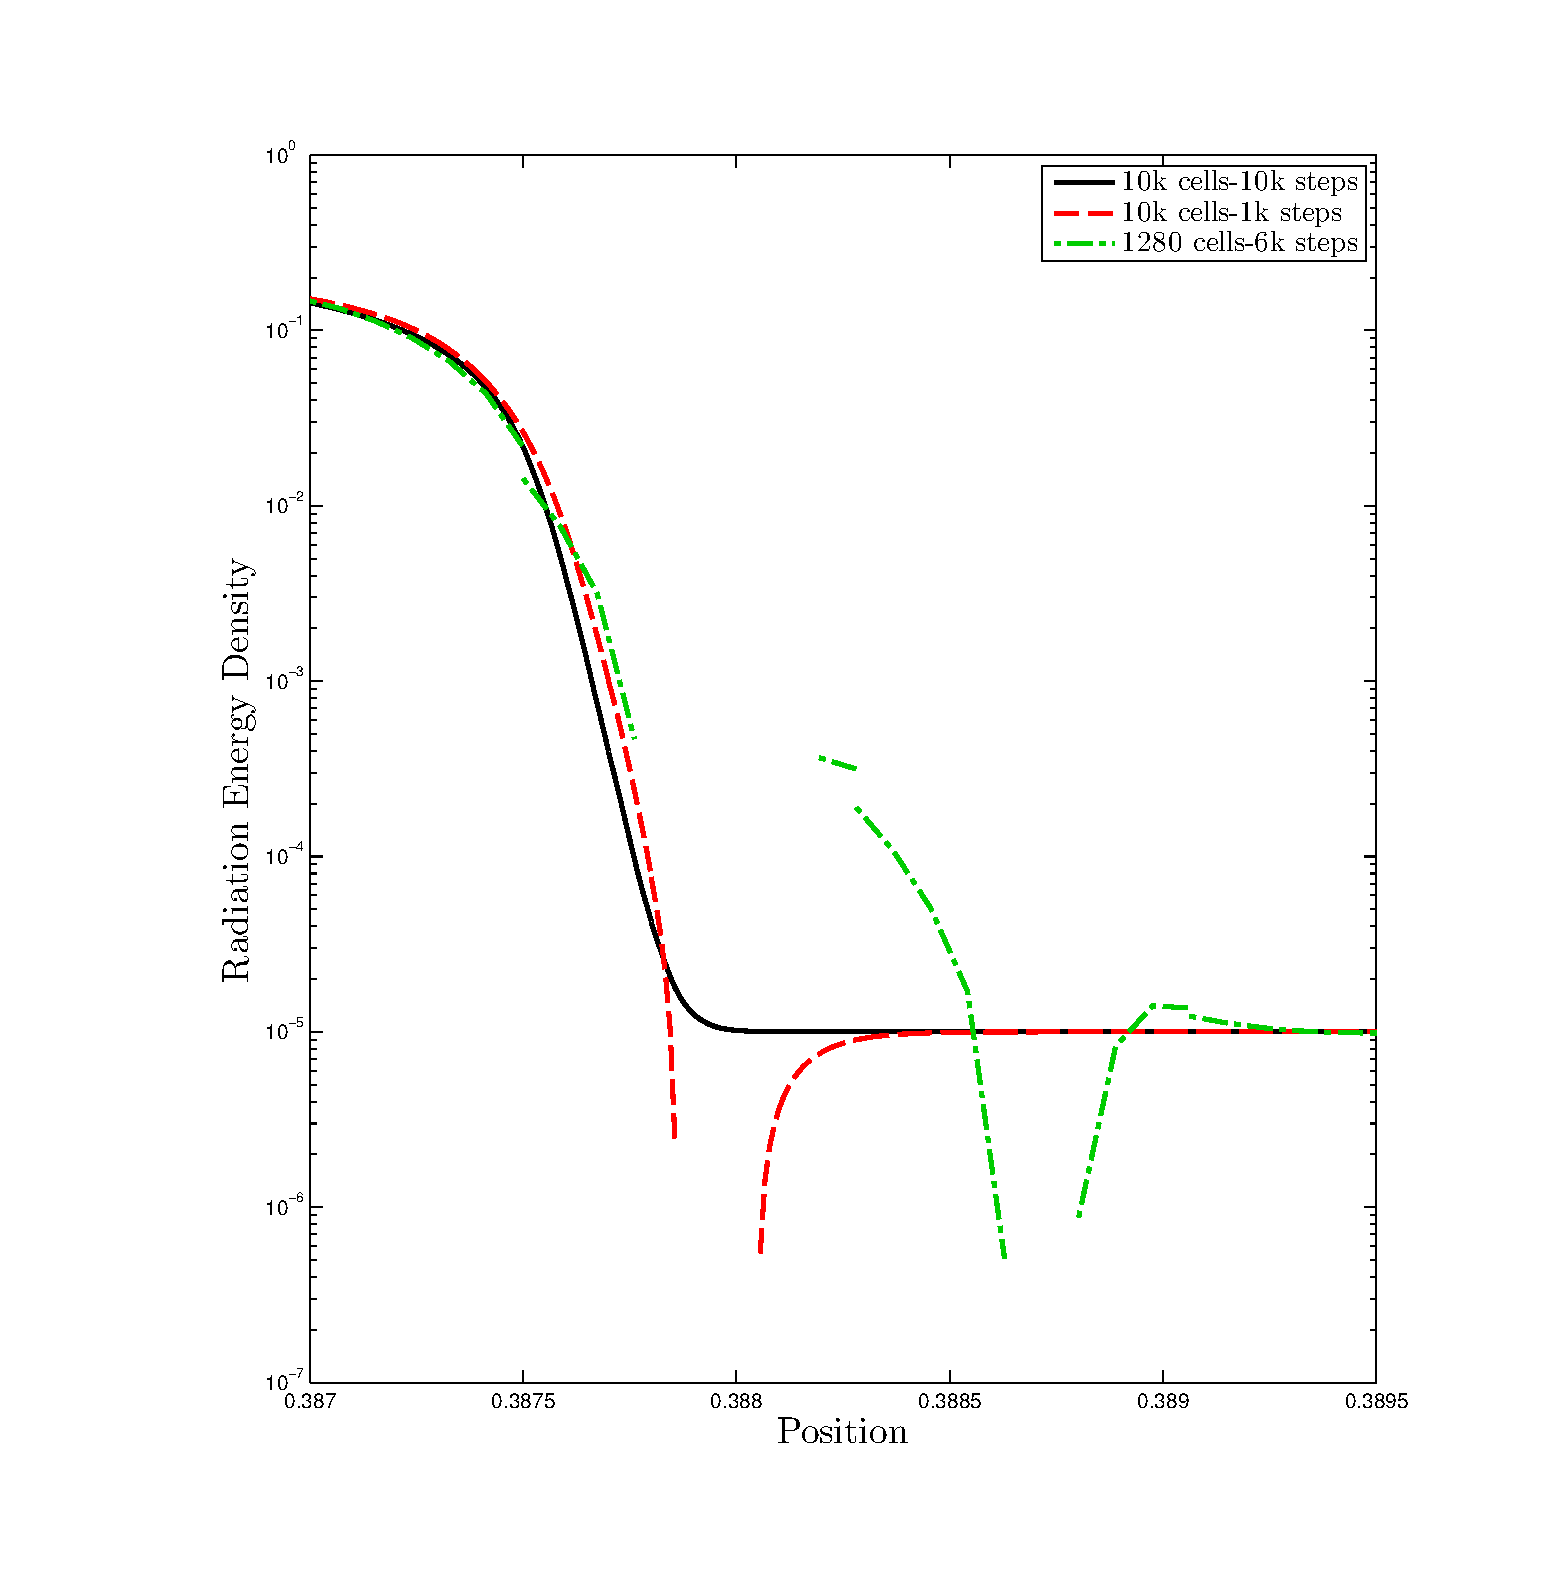
\includegraphics[height=0.8\textheight,trim=1.0in  0.75in 1.0in 1.0in,clip=true]{../chapter6_grey_radtran/Dissertation_Data/Zoom_10k_Phi.pdf}
\end{frame}

\begin{frame}
\frametitle{$S_2$ vs $S_8$}
\begin{columns}[t]
\column{0.5\textwidth}
\centering
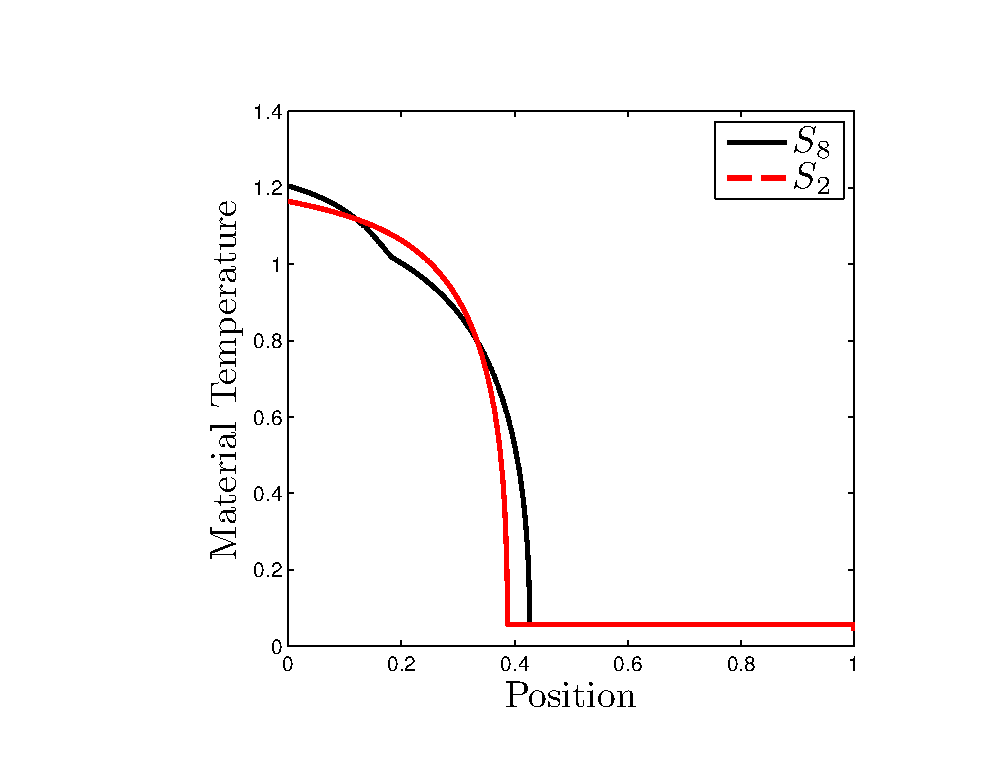
\includegraphics[width=2.5in,trim=1.0in  0.5in 0.2in 0.6in,clip=true]{../chapter6_grey_radtran/S8_vs_S2_Material_Temperature.pdf}
\column{0.5\textwidth}
\centering
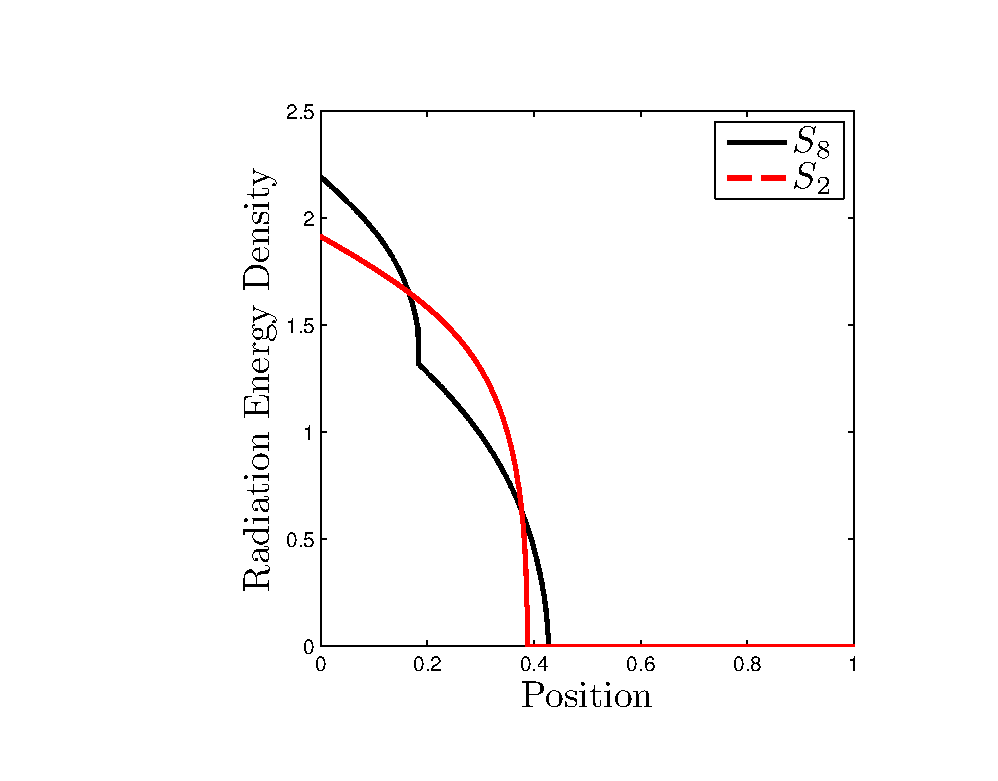
\includegraphics[width=2.5in,trim=1.0in  0.3in 0.2in 0.5in,clip=true]{../chapter6_grey_radtran/S8_vs_S2_Radiation_Energy_Density.pdf}
\end{columns}
\centering
5000 mesh cells, P4 SLXS Gauss, 5k time steps, 2-2 scheme
\end{frame}

\begin{frame}
\frametitle{$S_8$ Angular Intensity}
\centering
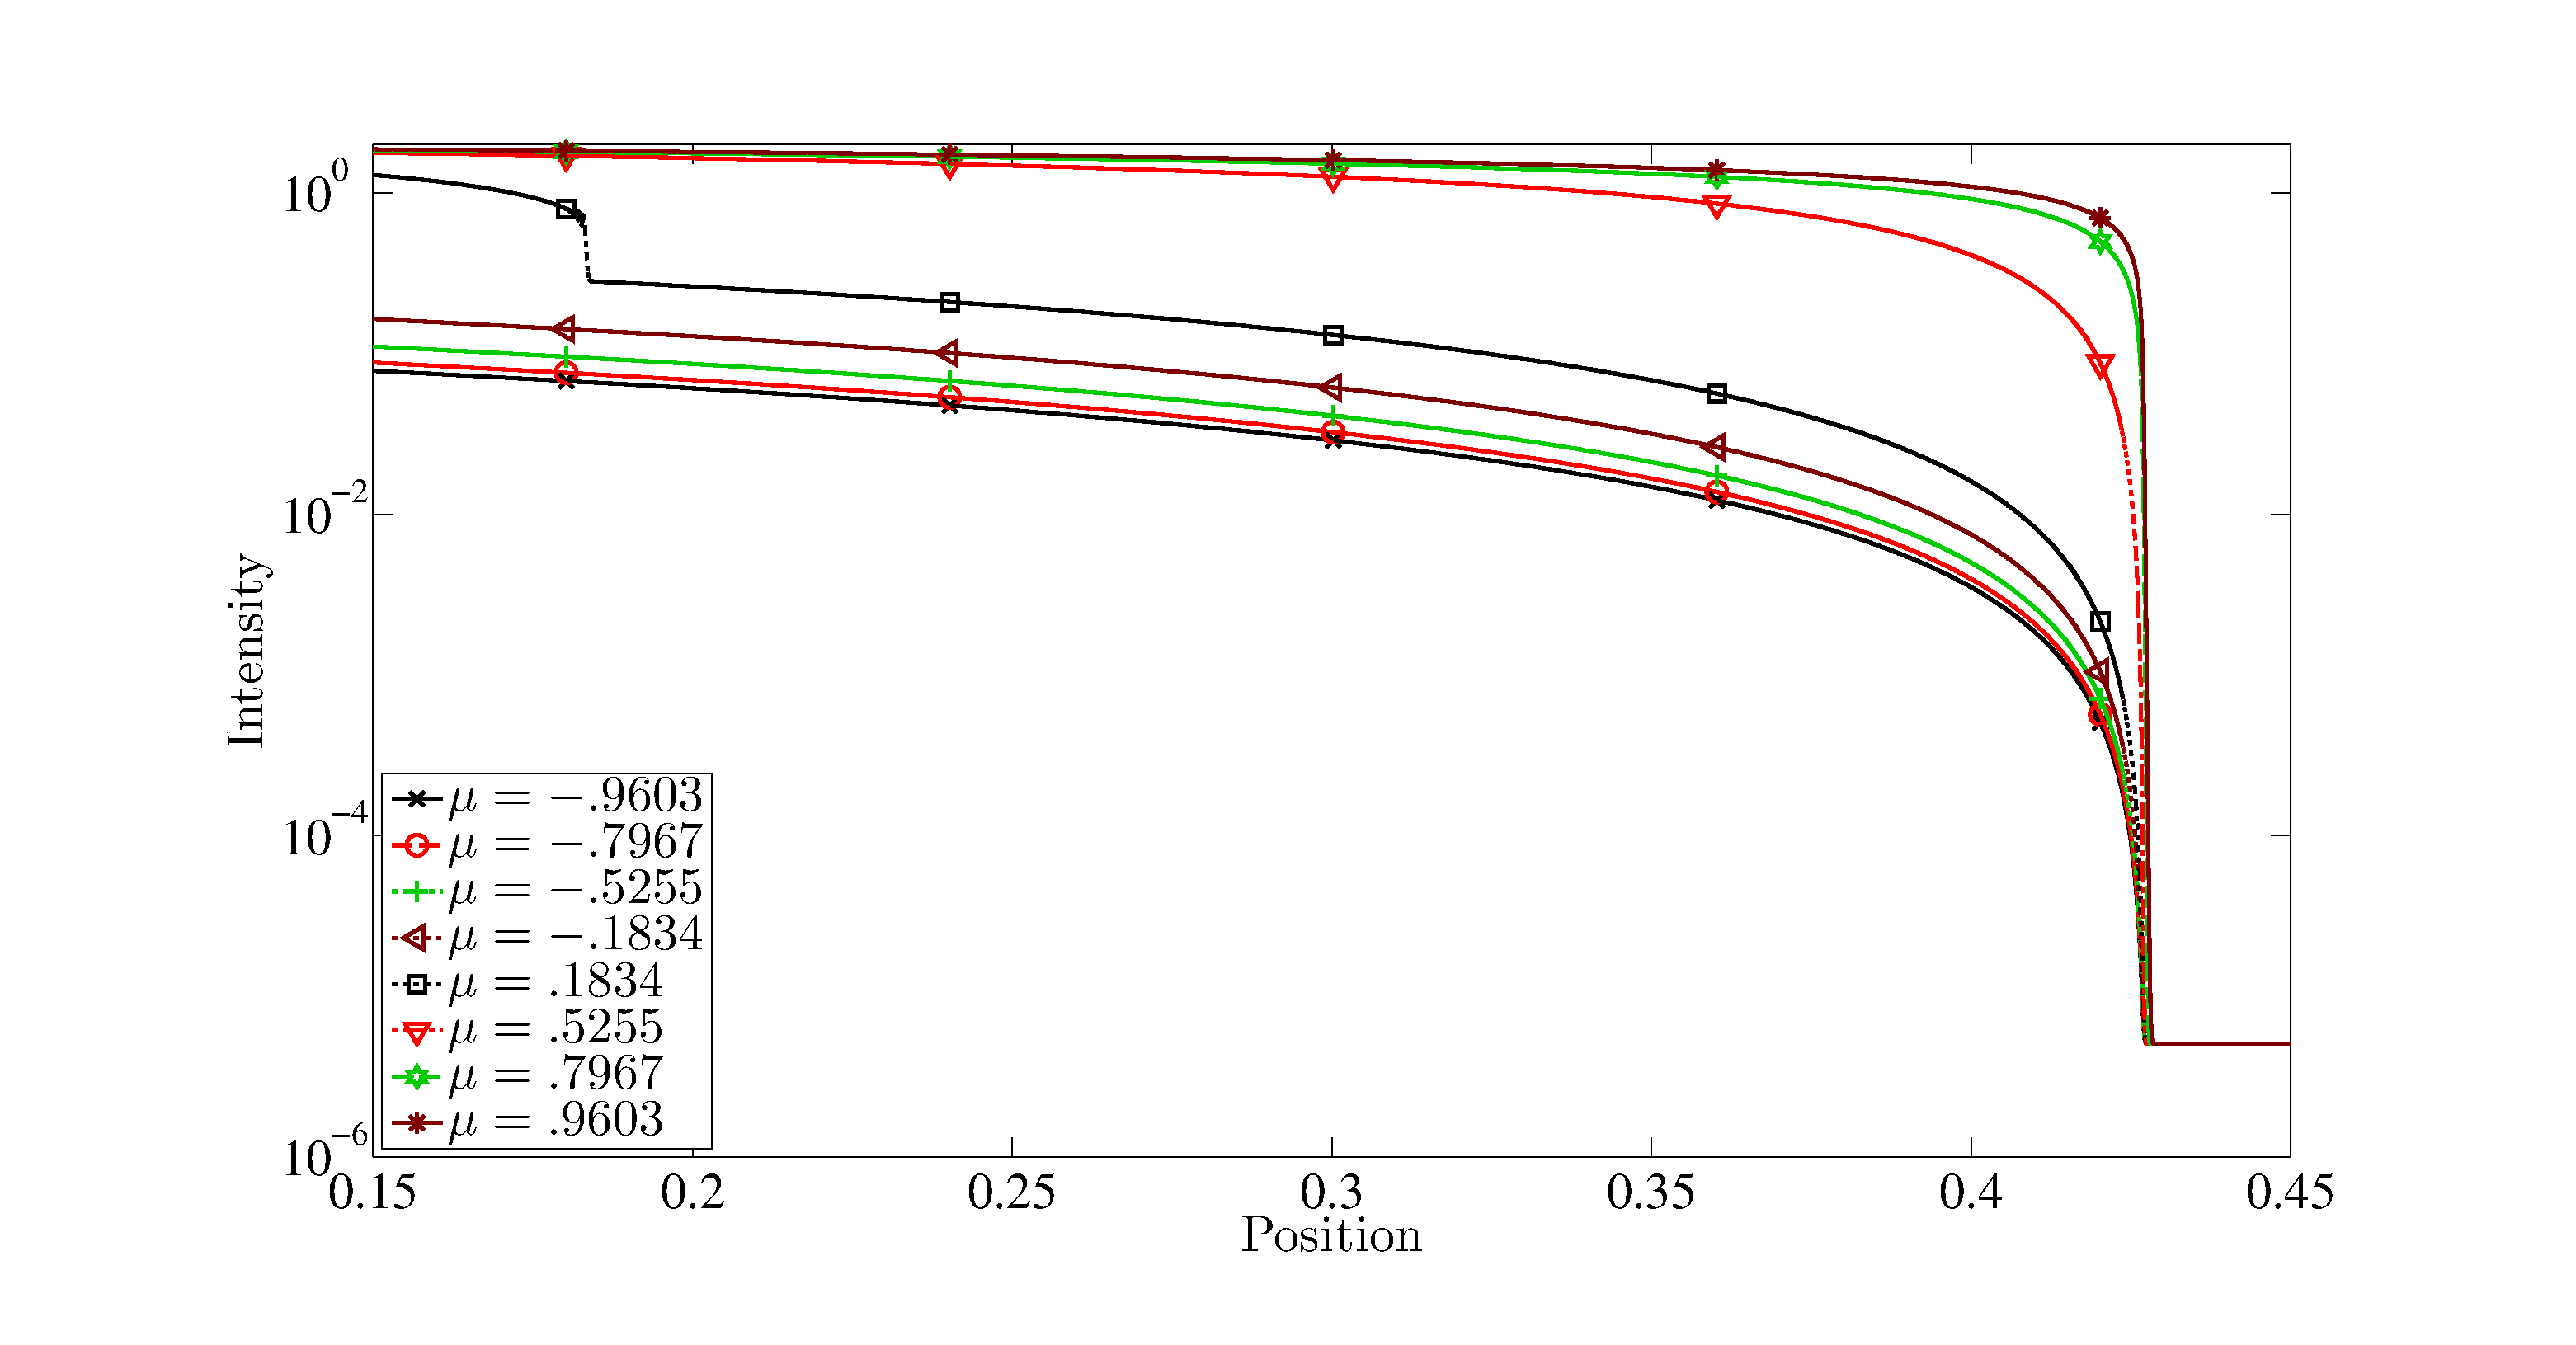
\includegraphics[width=\textwidth,trim=1.5in  0.5in 1.0in 1in,clip=true]{../chapter6_grey_radtran/S8_Intensity_SemiLogy.pdf}
\end{frame}

\begin{frame}
\frametitle{Wavefront Boundary Layers}
\centering
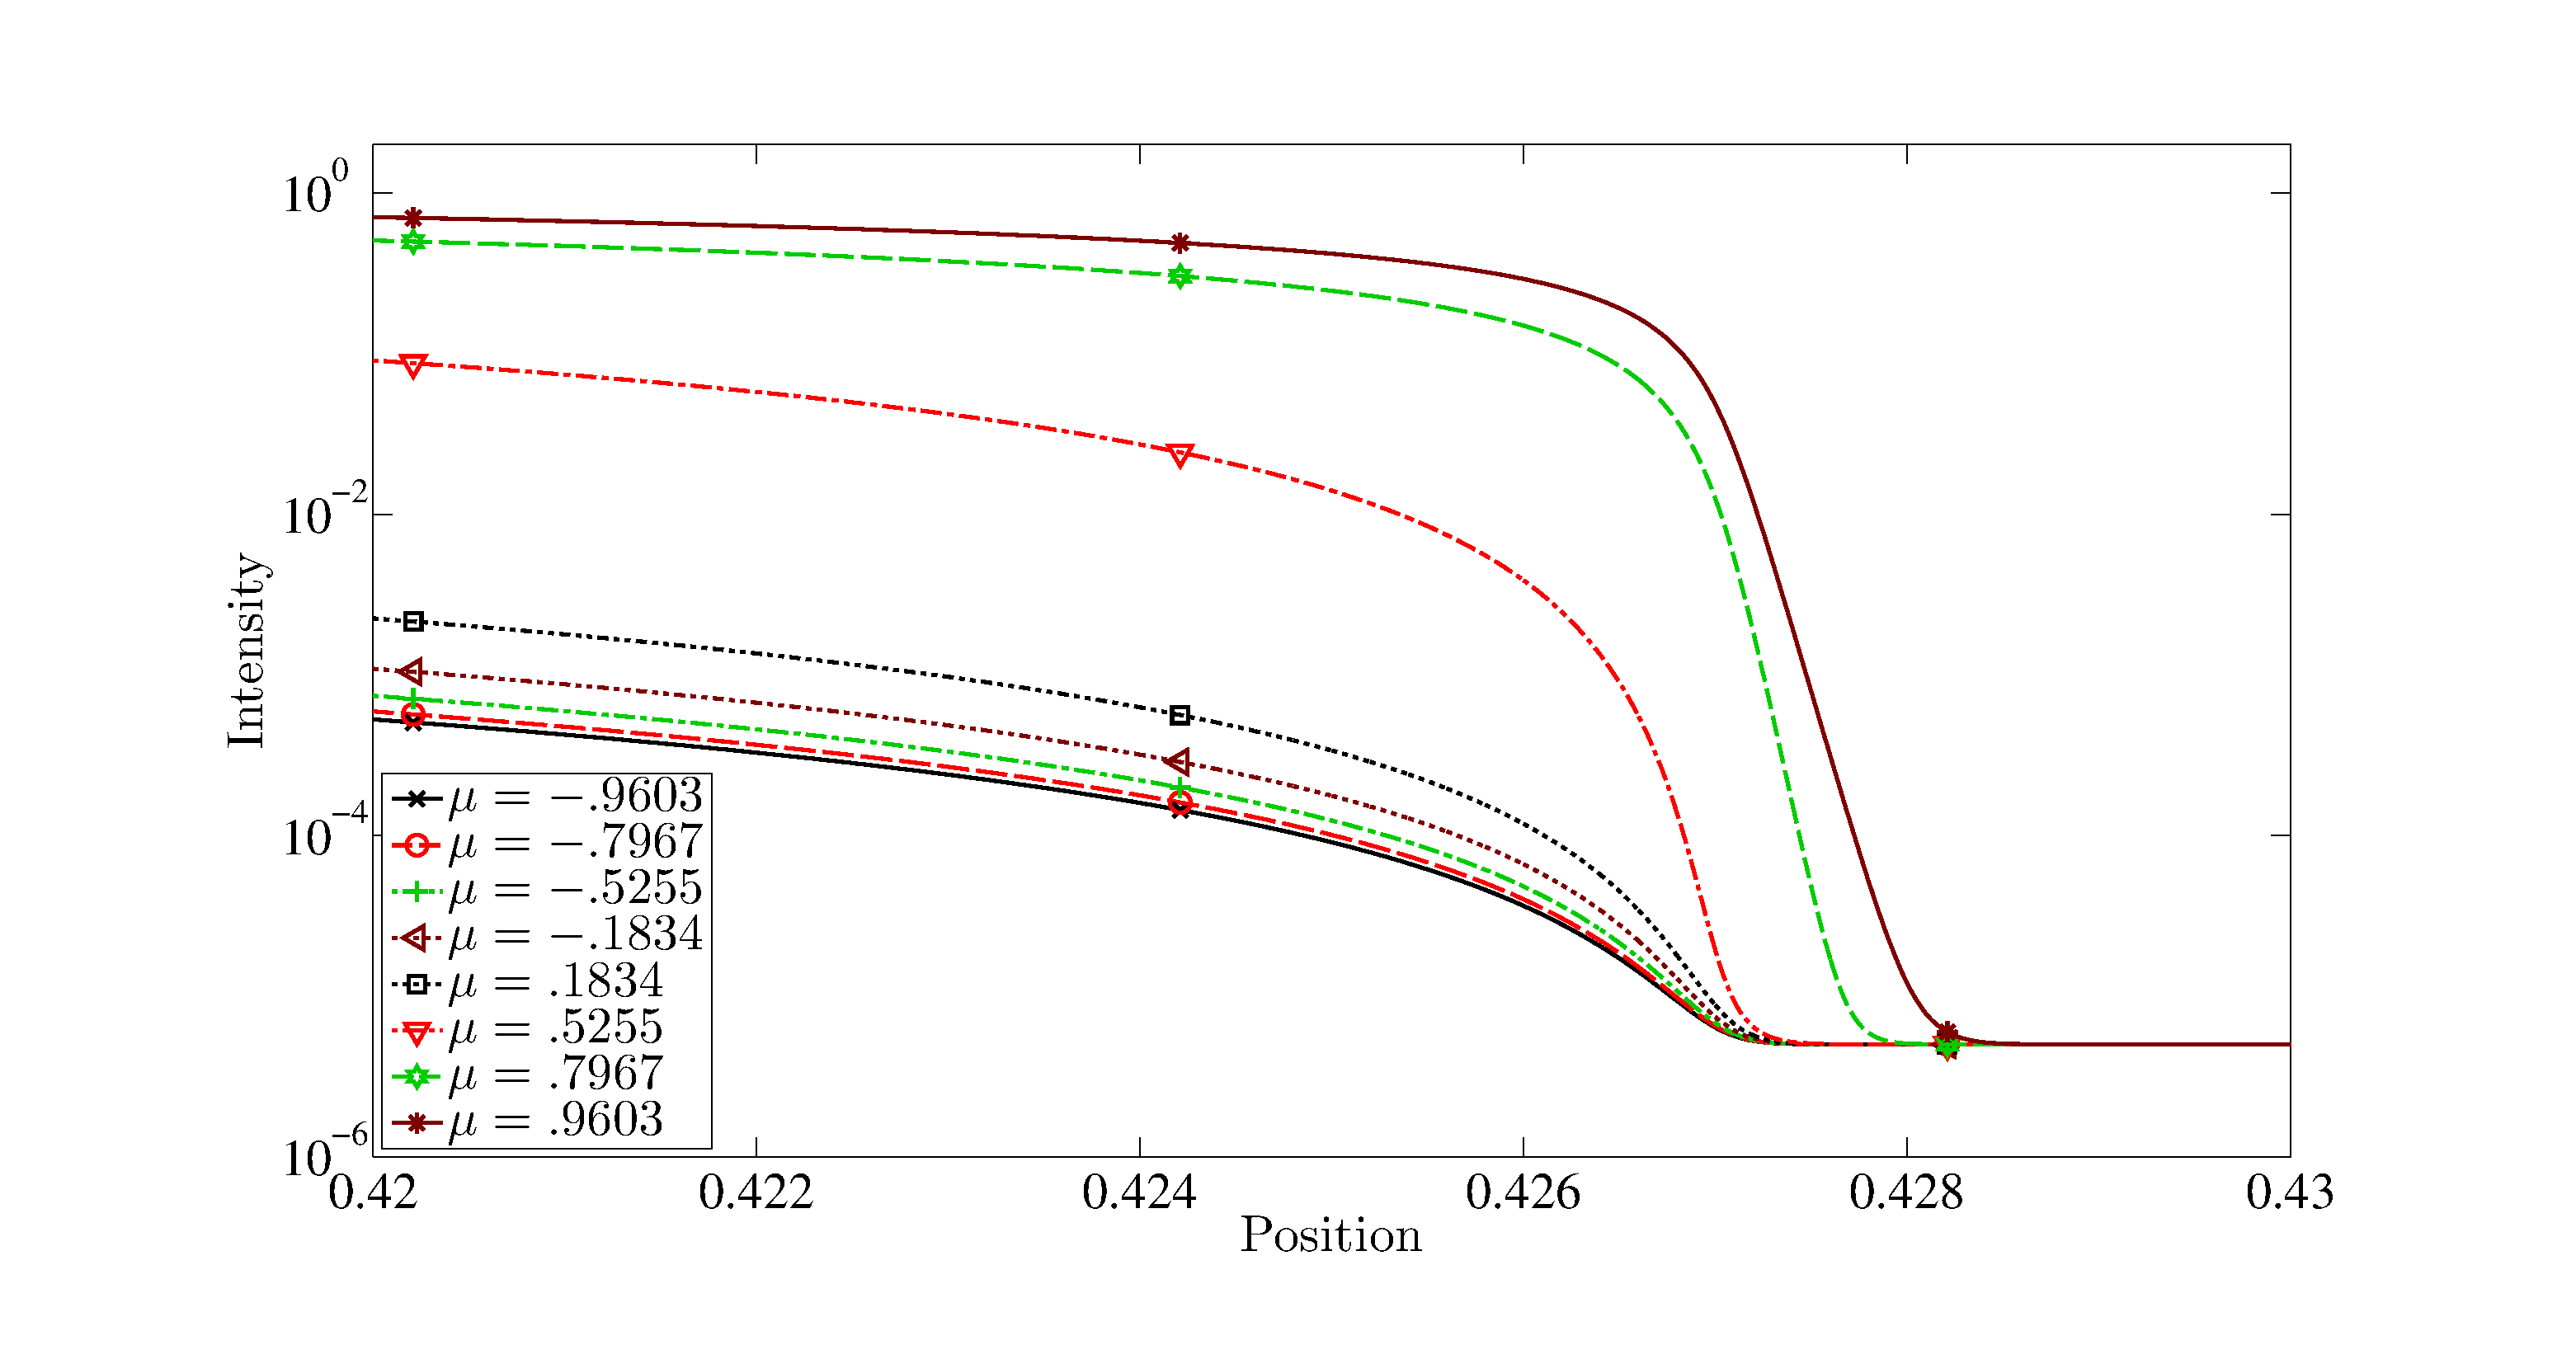
\includegraphics[width=1.05\textwidth,trim=1.75in  0.2in 1in 0.75in,clip=true]{../chapter6_grey_radtran/Dissertation_Data/S8_thermal_wavefront_boundary_layer.pdf}
\end{frame}

\begin{frame}
\frametitle{Need More Resolution for Interior Boundary Layer}
\centering
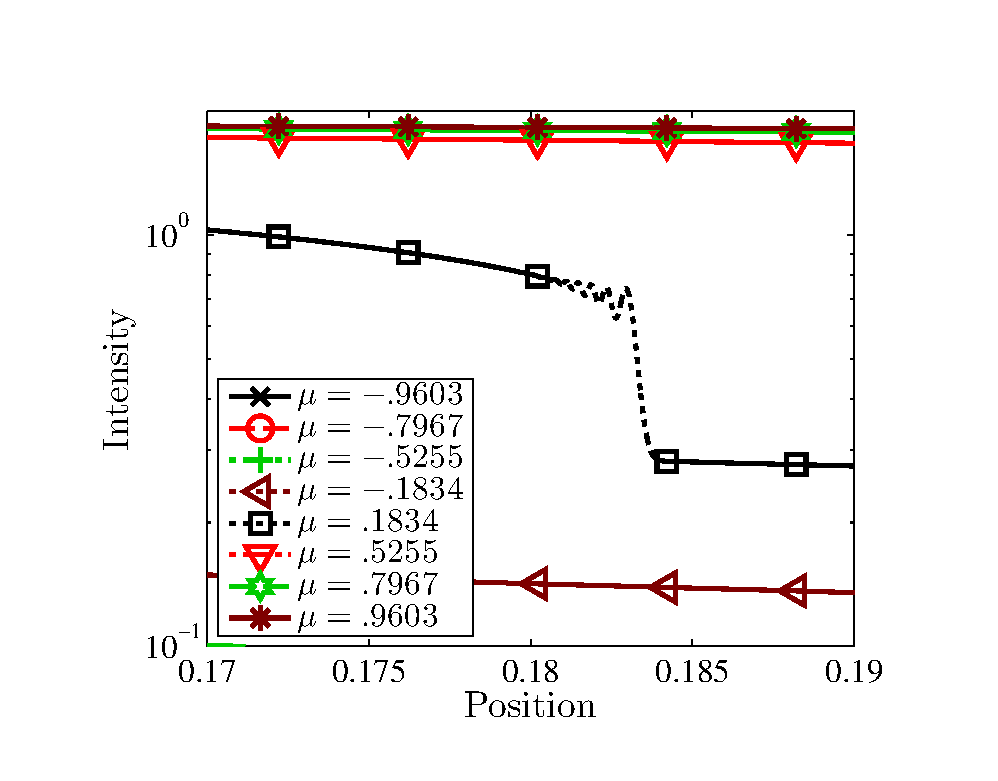
\includegraphics[height=0.8\textheight,trim=0.5in  0.2in 0.75in 0.5in,clip=true]{../chapter6_grey_radtran/Dissertation_Data/S8_pos_mu_glance_boundary_layer_log.pdf}
\end{frame}

\begin{frame}
\frametitle{$S_8$ vs $S_{32}$ Solutions}
\centering
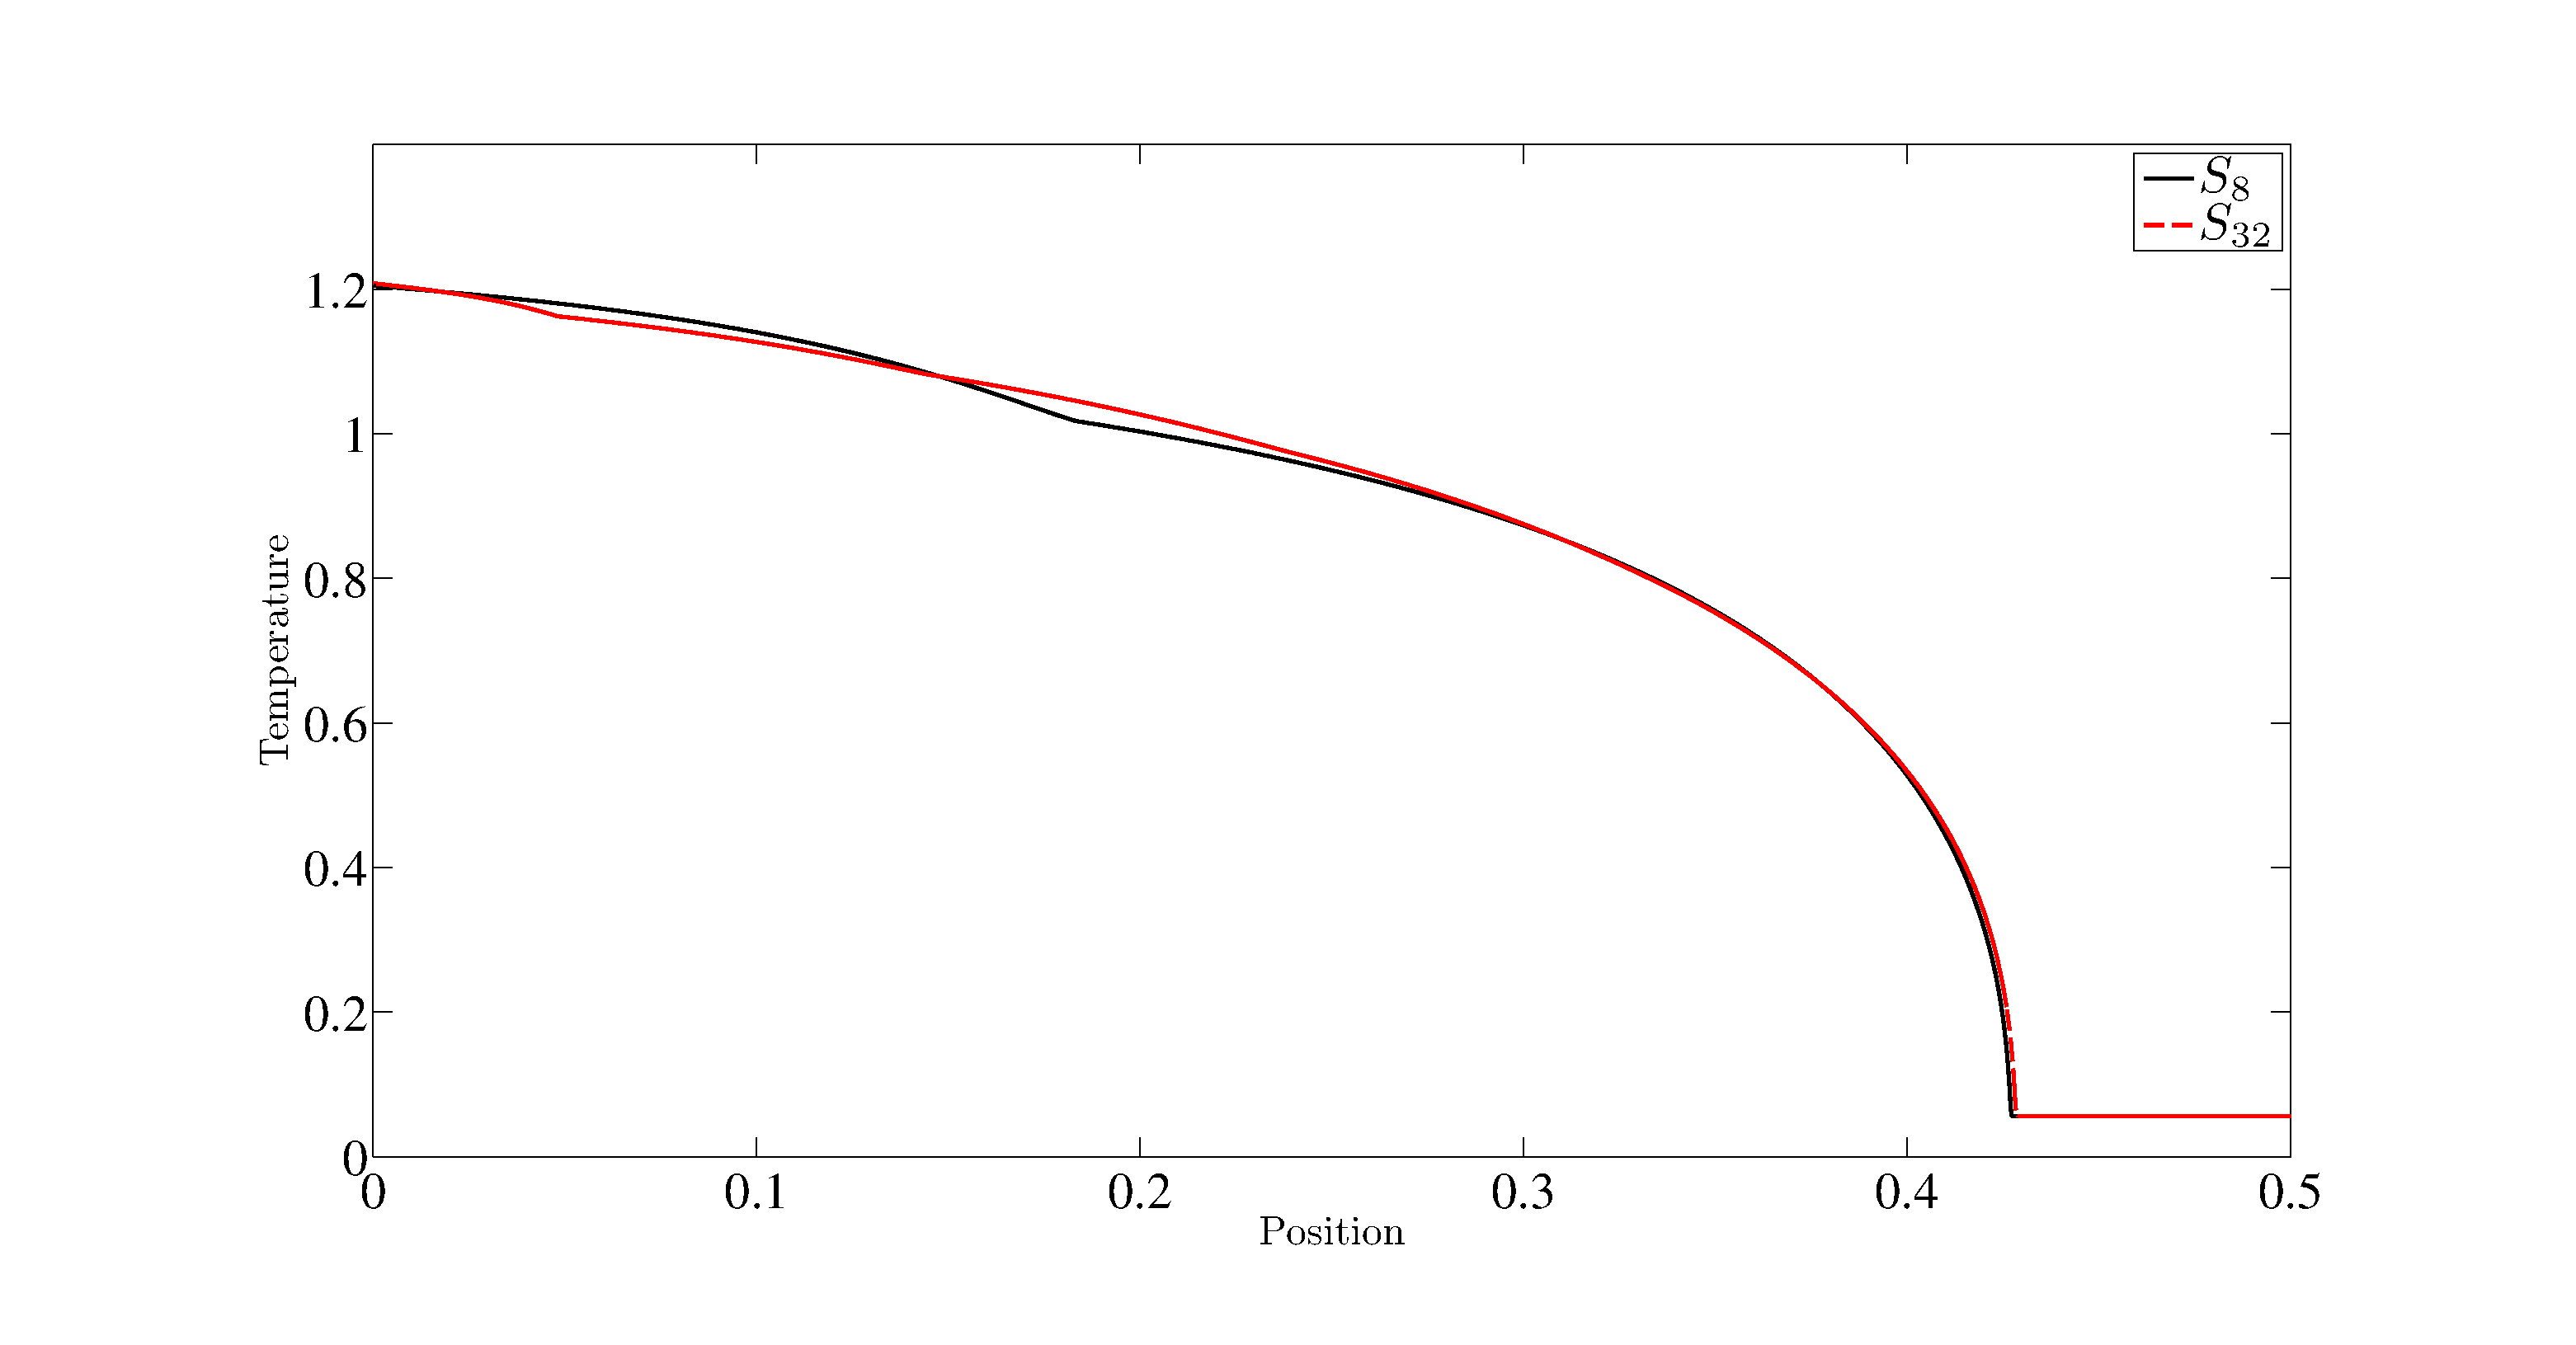
\includegraphics[width=0.75\textwidth,height=0.4\textheight,trim=1.5in  0.2in 0.5in 0.75in,clip=true]{../chapter6_grey_radtran/Dissertation_Data/S8_vs_S32_Material_Temperature.pdf}
%
\\
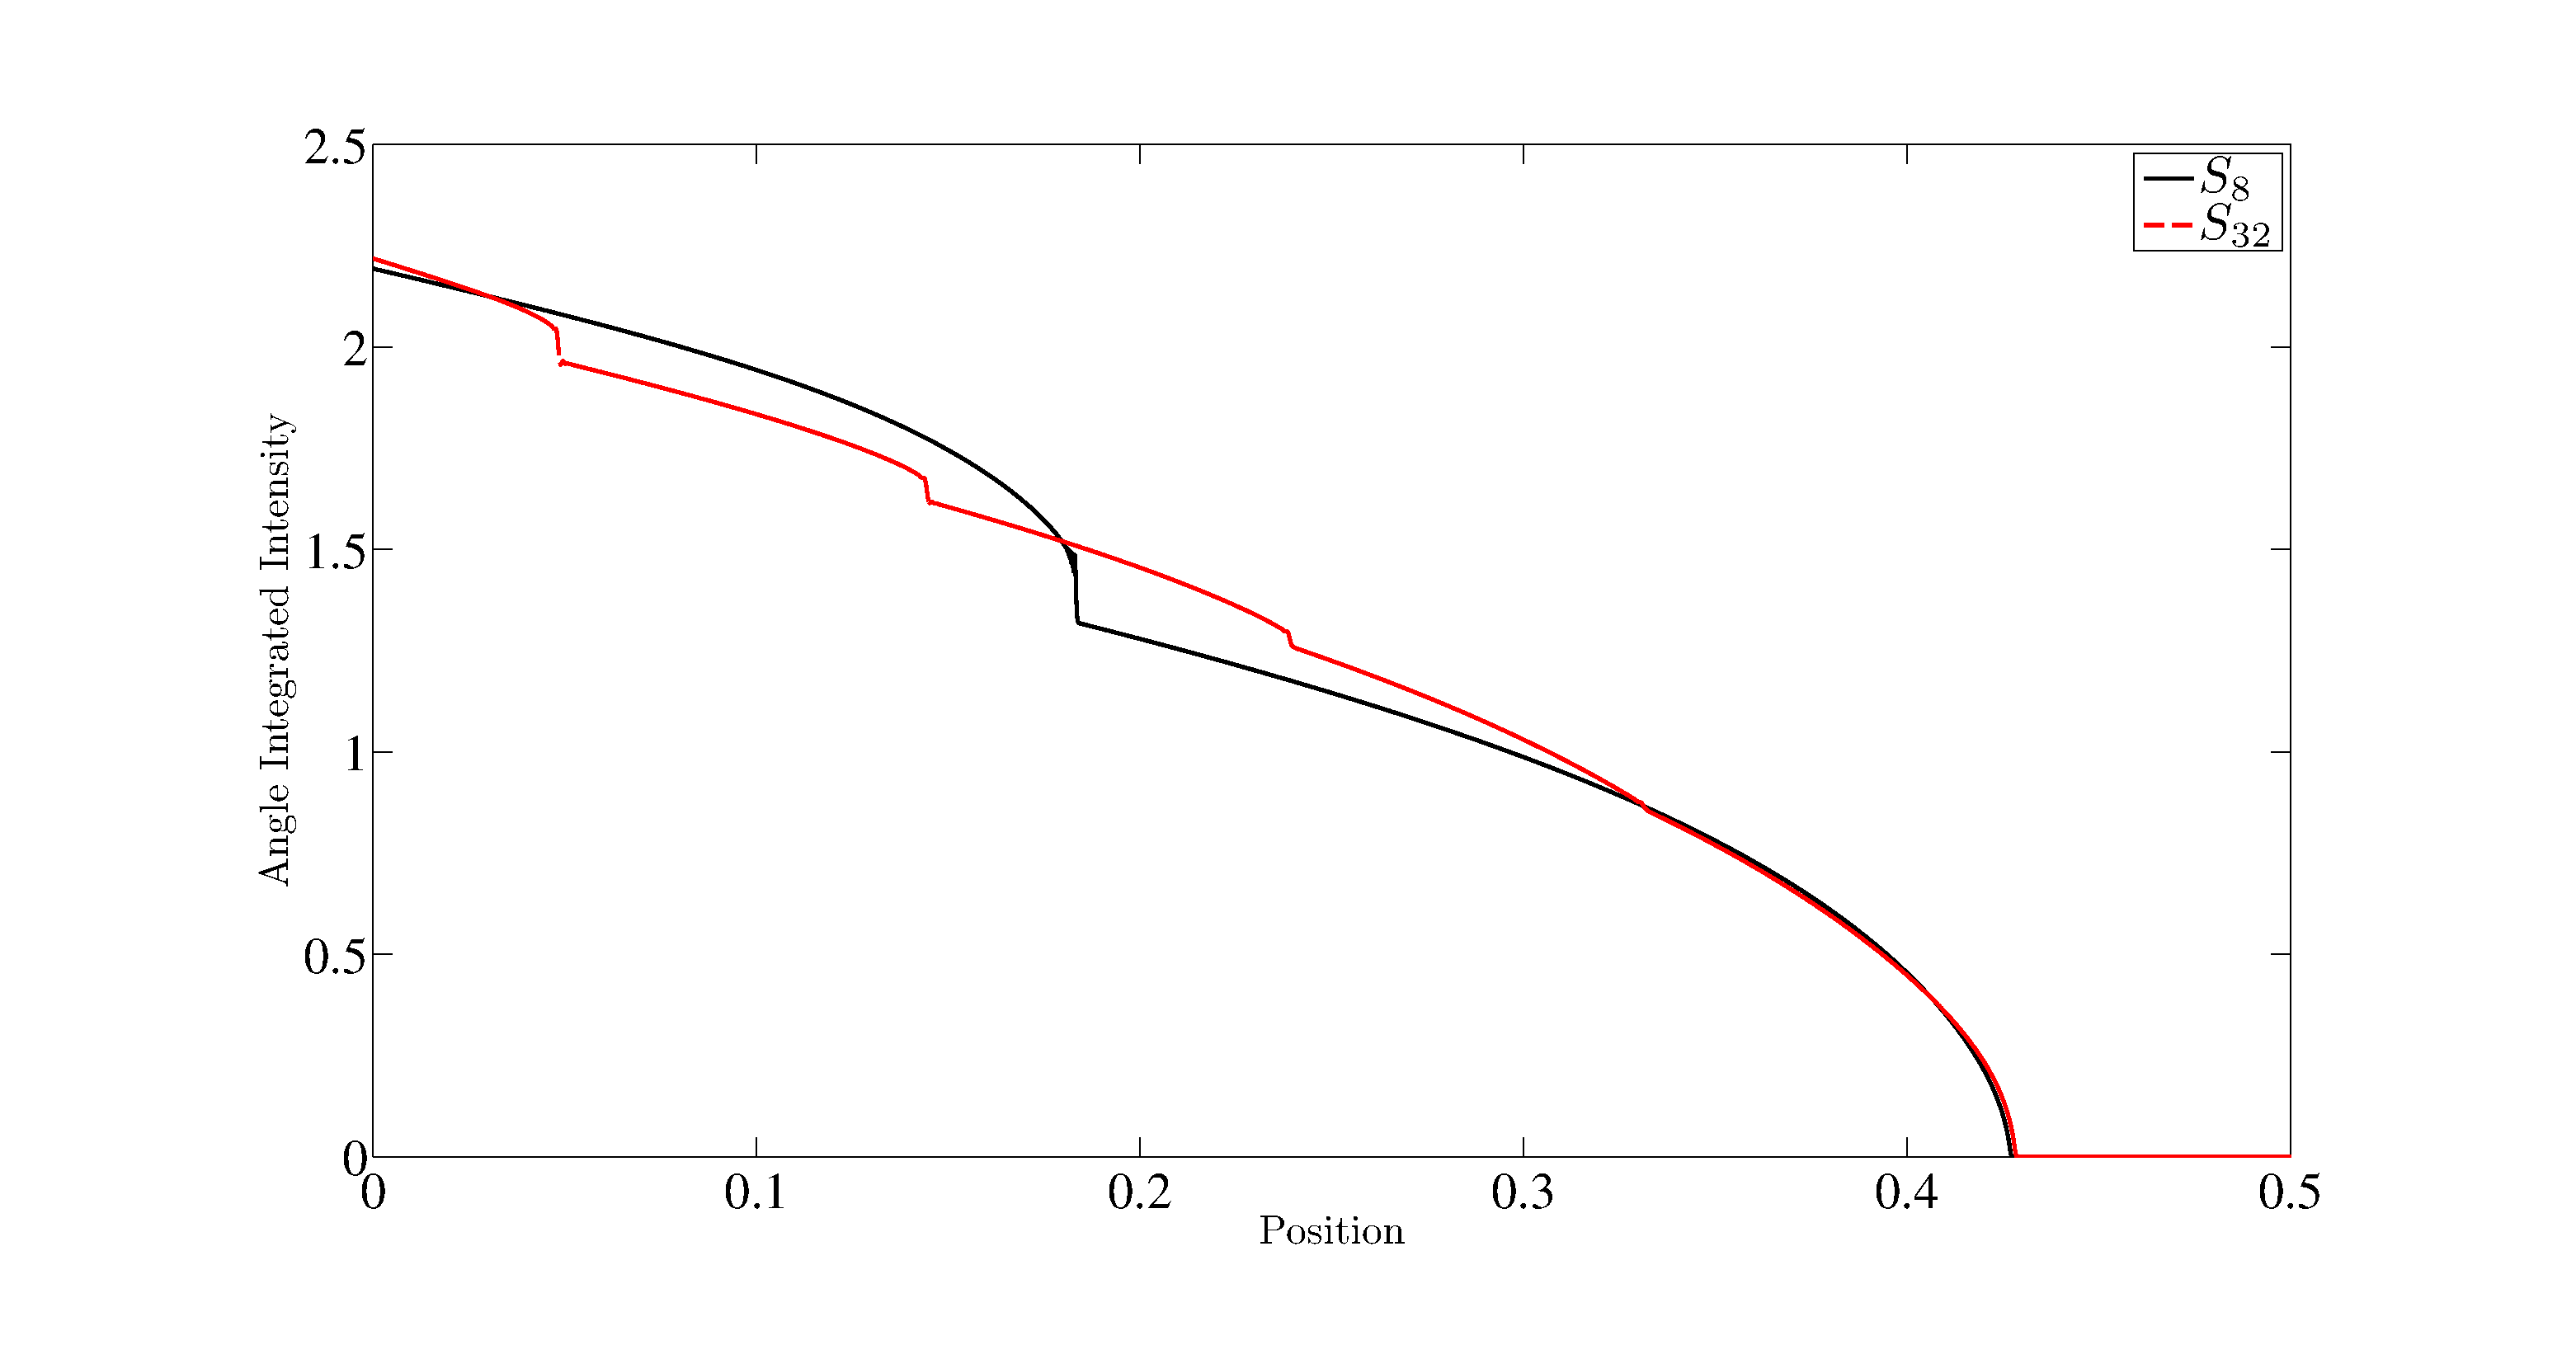
\includegraphics[width=0.75\textwidth,height=0.4\textheight,trim=1.5in  0.2in 0.5in 0.75in,clip=true]{../chapter6_grey_radtran/Dissertation_Data/S8_vs_S32_Radiation.pdf}
\\
$S_{32}$ solution- 1000 mesh cells, quartic SLXS Gauss, 5000 time steps
\end{frame}

\begin{frame}
\frametitle{$S_{32}$, $\mu_d > 0$ intensities}

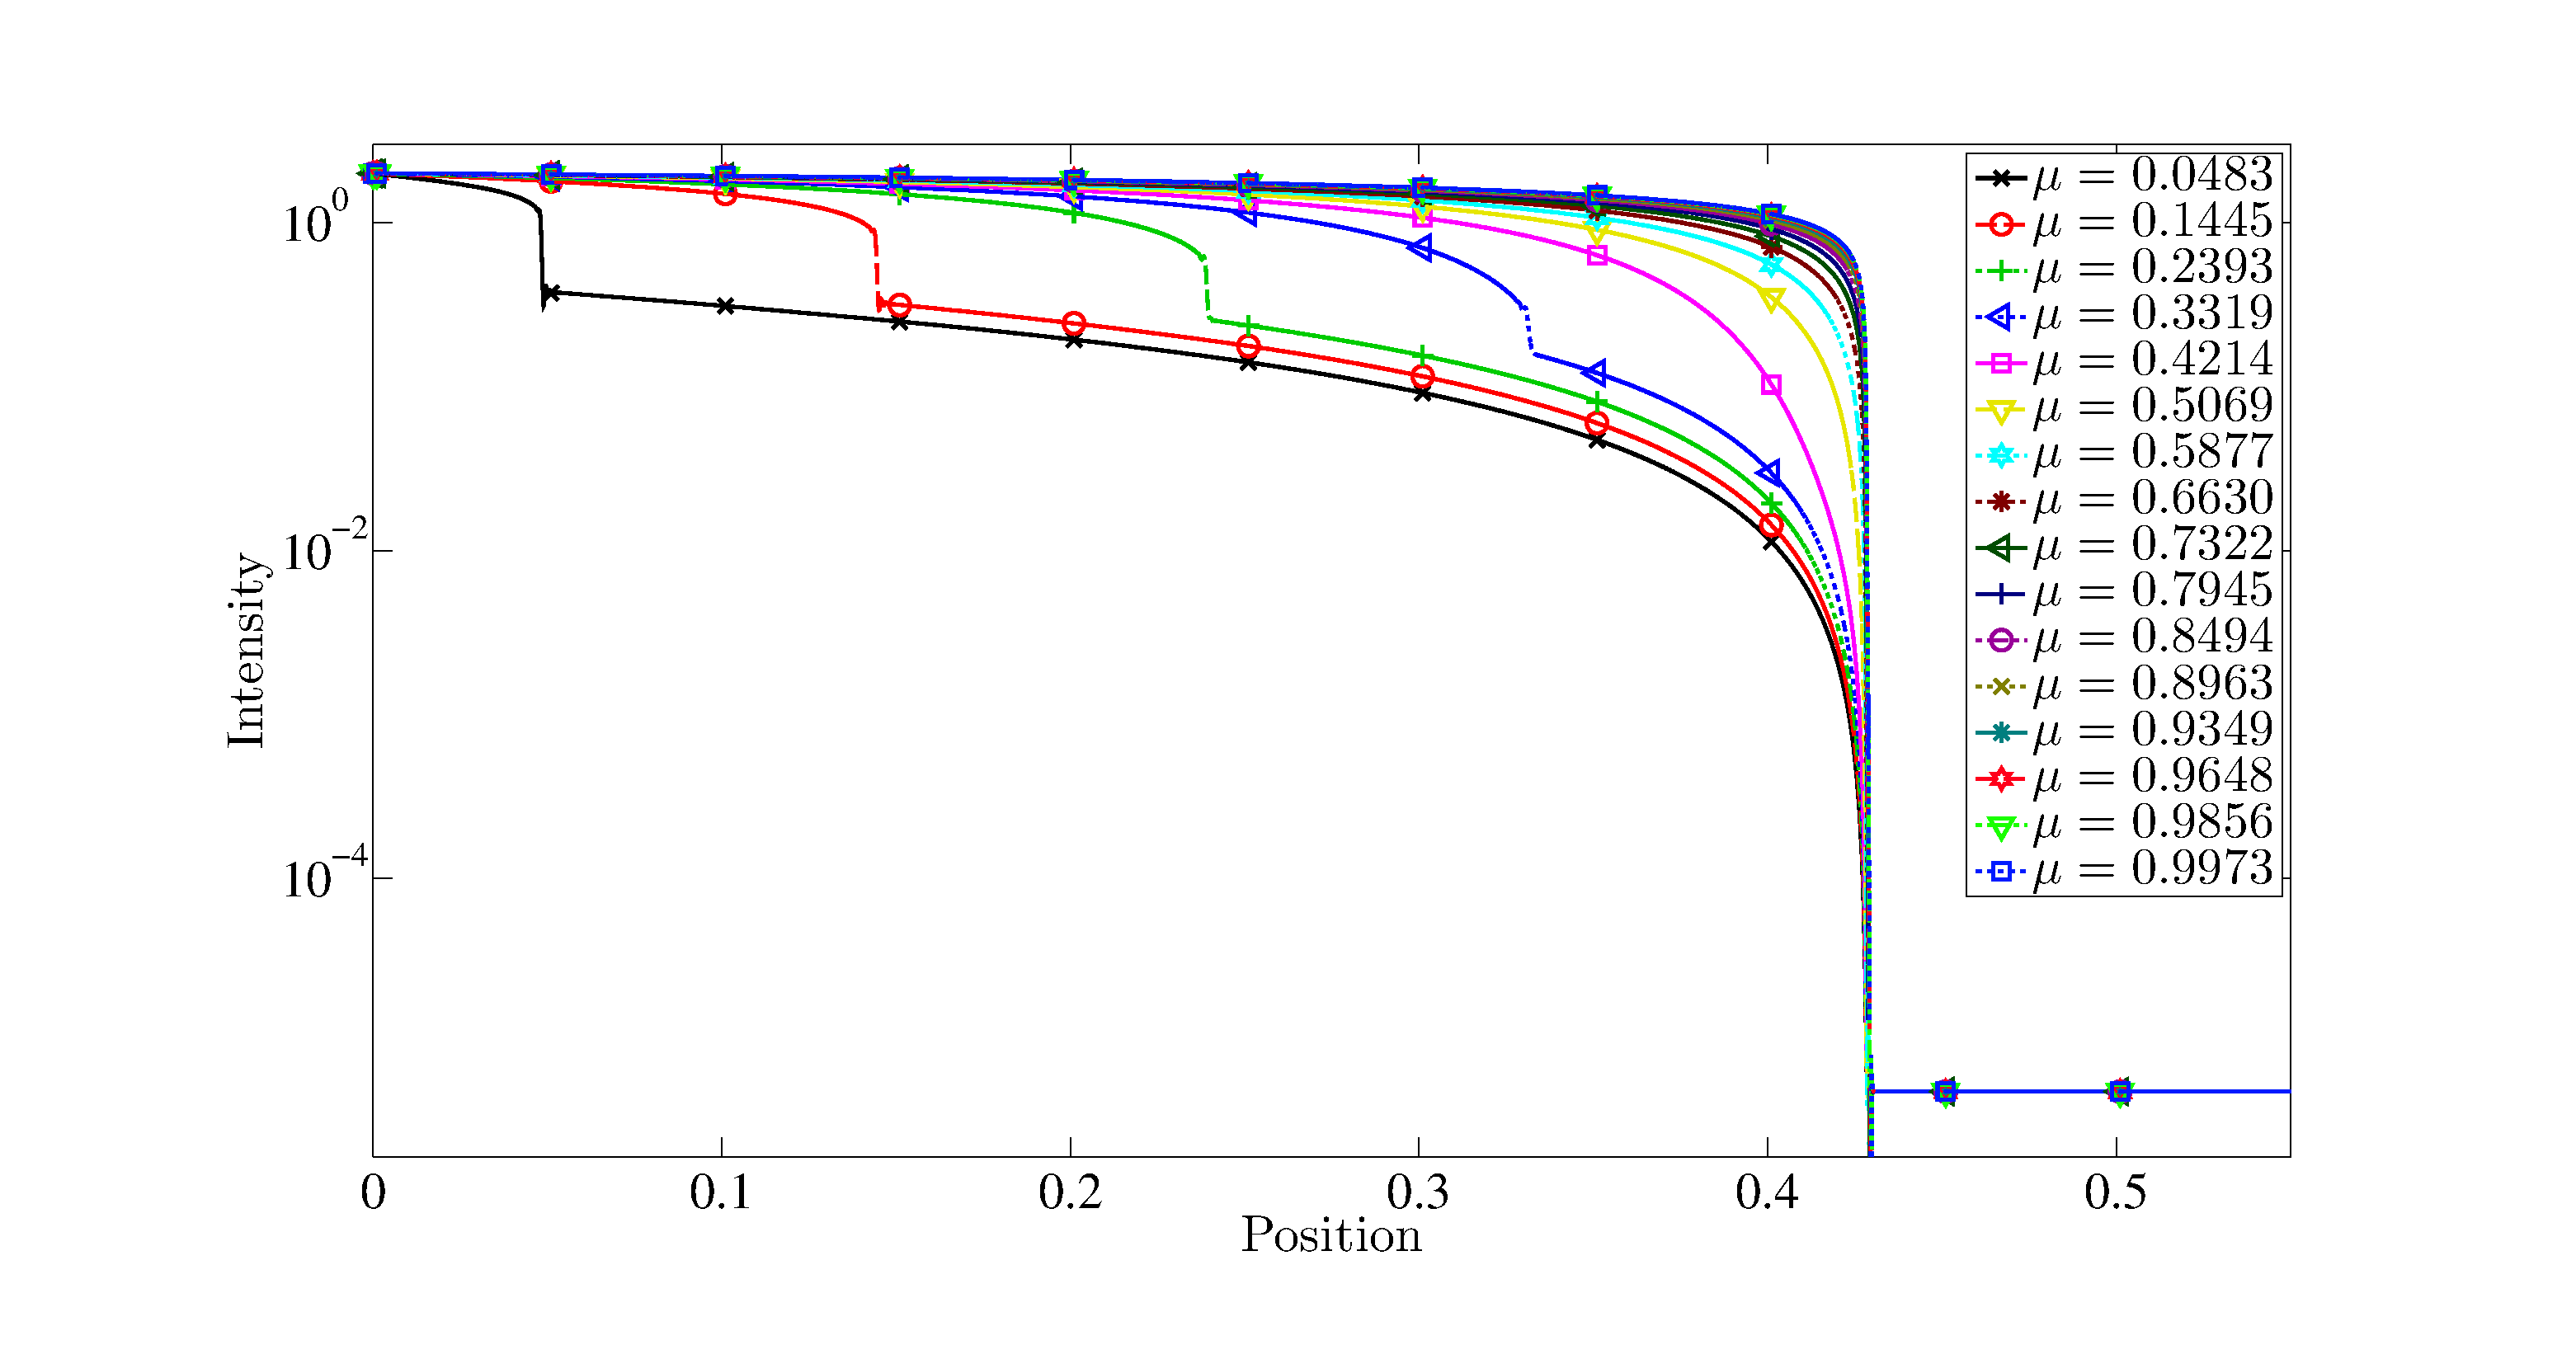
\includegraphics[width=\textwidth,trim=1.5in  0.2in 0.5in 0.75in,clip=true]{../chapter6_grey_radtran/Dissertation_Data/S32_Intensity.pdf}

\end{frame}

\section{Conclusions}
\subsection{Conclusions}
\begin{frame}
\frametitle{Conclusions}
In PhD we have
\begin{enumerate}
\item Developed a matrix lumping framework that is effective for arbitrary $P$
\item Demonstrated the need to consider spatial variation of material properties
\item Applied MIP diffusion operator to TRT acceleration
\end{enumerate}
Today we have
\begin{itemize}
\item Applied higher order DFEM to grey TRT
\item Examined the asymptotic accuracy of higher order DFEM for coupled grey TRT problems
\item Generated high resolution discrete ordinates results for grey TRT problems 
\end{itemize}
\end{frame}

\subsection{Long Term Future Work}
\begin{frame}
\frametitle{Potential Future Work}
\begin{itemize}
\item Complete multi-frequency capabilities
\item Diffusion limit analysis of higher order DFEM
\item Extend lumping framework to multiple spatial dimensions
\end{itemize}
\end{frame}

\subsection{Acknowledgments}
\begin{frame}
\frametitle{Acknowledgments}
Thanks for your time!
\vspace{0.3in}
Portions of this work were funded by the Department of Energy CSGF program, administered by the Krell Institute, under grant DE-FG02-97ER25308.
\\
\vspace{0.3in}
Additional support was provided by the Department of Energy, National Nuclear Security Administration, under Award Number(s) DE-NA0002376.

\end{frame}

%%%%%%%%%%%%%%%%%%%%%%%%%%%%%%%%%%%%%%%%%%%%%%%%%%%%%%%%%%%%%%%%%%%%%%%%%%%%%%%%%

\end{document}
%------------------------------------------------------------------------------